\chapter{Universal Constructions and Limits} 
    \section{Universal Morphisms}\label{section:universal_morphisms}

    This chapter is probably the most important chapter in these notes. 
    In an ideal world, this chapter would be the first chapter. 
    However, that would pedagogically go over terribly. The discussion requires 
    categories, functors, and natural transformations; we need the language 
    these concepts offer 
    to even begin to rigorously define what a universal construction even is. 

    But at this point, we are in fact equipped with the fundamentals. So we can now 
    go on and define what a universal construction is, and demonstrate its prevalence 
    in mathematics and therefore the usefulness of category theory as a convenient language 
    to discuss these concepts. 

    To begin, we will motivate with a few examples.

    Let $\phi, \psi: (G, \cdot)  \to (H, +)$ be a pair of abelian\footnote{The abelian-ness becomes important later.} 
    group homomorphisms. We now ask the question:
    \begin{center}
        \textcolor{NavyBlue}{What is the set of all $g \in G$ such that $\phi(g) = \psi(g)$? Is it a subgroup of $G$?}
    \end{center}
    To determine this, it is equivalent to asking when $\phi(g) - \psi(g) = 0 
    \implies (\phi - \psi)(g) = 0$. Hence every such $g \in G$ lies in the kernel of 
    $\phi - \psi: G \to H$, and every element in the kernel is such a desired element; so 
    we've answered the first question. The kernel is a subgroup of $G$, so we've answered the last question. 
    Now because this is a kernel, it has an inclusion 
    homomorphism $i: \ker(\phi - \psi) \to G$. So far, our picture looks like this:
    \begin{center}
        \begin{tikzcd}
            \ker(\phi - \psi)
            \arrow[r, "i"]
            &
            G 
            \arrow[r, shift left = 0.5ex, "\phi"]
            \arrow[r, shift left = -0.5ex, swap, "\psi"]
            &
            H
        \end{tikzcd}
    \end{center}
    and clearly $\phi \circ i = \psi \circ i$. 
    Now suppose that $\sigma: K \to G$ is another group homomorphism with the property 
    that $\phi \circ \sigma = \psi \circ \sigma$. Then by our previous work, this means 
    that for each $k \in K$, we have that $\sigma(k)\in\ker(\phi - \psi)$. That is, 
    \[
        \im(\sigma) \subset \ker(\phi - \psi)  
    \]
    Hence instead of mapping $K$ into $G$, we can instead map $K$ into $\ker(\phi - \psi)$, 
    and then travel back to $G$ using $i$.
    So, there is \textbf{a unique} morphism $\tau: K \to \ker(\phi - \psi)$
    such that the diagram below commutes (Prove it is unique; it shouldn't be too bad).
    \begin{center}
        \begin{tikzcd}[column sep = 1.4cm, row sep = 1.4cm]
            \ker(\phi - \psi)
            \arrow[r, "i"]
            &
            G 
            \arrow[r, shift left = 0.5ex, "\phi"]
            \arrow[r, shift left = -0.5ex, swap, "\psi"]
            &
            H
            \\
            K
            \arrow[u,  dashed, "\tau"] 
            \arrow[ur, swap, "\sigma"]
            &
            &
        \end{tikzcd}
    \end{center}    
    What's really going on? This is an example of a universal construction. We have a 
    ``supreme'' morphism $i: \ker(\phi -\psi) \to G$ with the property that $\phi \circ i = \psi \circ i$.
    Any other morphism $\sigma: K \to G$ with the same property that $\phi\circ\sigma = \psi \circ \sigma$ 
    must factor through the ``supreme'' morphism $i$ \textbf{in a unique way}. Uniqueness here is 
    very important. 

    Now, if you haven't seen this definition before, it's going to sting a little, 
    and you'll probably have to read it 20 times and do many, many examples (not just 
    \emph{look} at examples, you have to \emph{do} some yourself) to 
    achieve true understanding. But here we go:

    \begin{definition}\label{definition:universal_morphism_from_D_to_F}
        Let $F: \cc \to \dd$ be a functor and $D$ an object of $\dd$.
        Define a \textbf{universal morphism from $\bm{D}$ to $\bm{F}$} 
        to be a morphism
        \[
            \textcolor{red}{u}: D \to F(\textcolor{NavyBlue}{C})
        \]
        with $\textcolor{NavyBlue}{C} \in \ob(\cc)$ and 
        $\textcolor{Red}{u}$ a morphism in $\dd$ equipped with the \textbf{universal property:}
        \begin{center}
            \begin{minipage}{0.8\textwidth}
            For every morphism $f: D \to F(C')$, there 
            exists a \textbf{unique} morphism $h: \textcolor{NavyBlue}{C} \to C'$ 
            such that the diagram below commutes. 
            \end{minipage}
            \begin{center}
                \begin{tikzcd}[row sep = 1.4cm, column sep = 1.4cm]
                    D \arrow[r, Red, "u"] \arrow[dr, swap, "f"] & F(\textcolor{NavyBlue}{C})\arrow[d, dashed, "F(h)"] \\
                    & F(C') 
                \end{tikzcd}
                \hspace{1cm}
                \begin{tikzcd}[row sep = 1.4cm, column sep = 1.4cm]
                    \textcolor{NavyBlue}{C} \arrow[d, dashed, "h"]\\
                    C'
                \end{tikzcd}
            \end{center}
        \end{center}
        The arrow $h$ is dashed, and should be read as 
        "there exists an $h$.'' This is a practice 
        that we will continue to use throughout this text. 
    \end{definition}

    \begin{remark}
        To the beginner, this definition will most likely make zero sense. 
        The only way that it will make sense is to see the definition in action.
    \end{remark}

    A universal arrow can also be thought of as a pair $(\textcolor{NavyBlue}{C}, \textcolor{red}{u}: D \to F(\textcolor{NavyBlue}{C}))$.
    This just emphasizes that $\textcolor{NavyBlue}{C}$ is special. 
    This isn't really useful for us to imagine in this way right now. 
    So you don't have to think of it as a pair, so long as you remember you're mapping to
    $F(\textcolor{NavyBlue}{C})$. 

    The point is that \textit{any} arrow of the form $f: D \to F(C')$
    forces the \textit{unique} existence of an arrow $f' : C \to C'$
    such that $F(h) \circ \textcolor{Red}{u} = f$.  

    \begin{example}
        Let $V$, $W$ be finite-dimensional vector spaces over a field $k$. Denote their 
        bases as $\{v_1,  v_2, \dots, v_n\}$ and $\{w_1, w_2, \dots, w_m\}$. 
        \begin{center}
            \begin{minipage}{0.8\textwidth}
                \textbf{Q:} What does it take for a function $T: V \to W$ to be a linear transformation? 
            \end{minipage}
        \end{center}
        Well, suppose we have a linear transformation. Since each element of 
        $V$ may be written as $c_1v_1 + \cdots + c_nv_n$  for $c_i \in k$, we 
        see that 
        \[
            T(c_1v_1 + \cdots + c_nv_n) = c_1T(v_1) + \cdots + c_nT(v_n).
        \]
        Thus we have an answer. 
        \begin{center}
            \begin{minipage}{0.8\textwidth}
                \textbf{A:} To define a linear transformation $T: V \to W$, it suffices to specify 
                where we want $T$ to send the basis elements $v_1, \dots, v_n$.
            \end{minipage}
        \end{center}
        An illustration of this fact is below. 
        \begin{center}
            \begin{tikzpicture}[>=stealth]
                \node at (-2.25, 2.7) {$\rr^3$};
                \tdplotsetmaincoords{70}{120}
                \begin{scope}[tdplot_main_coords]
                    % axes
                    \pgfmathsetmacro{\scale}{5} % axes length
                    \coordinate (O) at (0, 0, 0);         % origin
                    \coordinate (Y) at (0, \scale-1, 0);    % y axes
                    \coordinate (Z) at (0, 0, \scale-2);  % z axes
                    \coordinate (X) at (\scale, 0, 0);    % x axes
        
        
                    % axes labels
                    \draw[semithick, ->] (O) -- (Y) node[right] {$y$};
                    \draw[semithick, ->] (O) -- (Z) node[above] {$z$};
                    \draw[semithick, ->] (O) -- (X) node[below] {$x$};
        
        
                    \draw[-stealth, thick, red] (0,0,0) -- (0, 0, 2);
                    \draw[-stealth, thick, Green!80!black] (0, 0, 0) -- (2, 0, 0);
                    \draw[-stealth, thick, blue] (0, 0, 0) -- (0, 2, 0);
        
                \end{scope}
                \draw[->] (2,2) to[bend left] (5,2);
                
                \begin{scope}[xshift = 9cm, yshift = 1cm]
                    \node at (-2.15, 1.8) {$P_n(x)$};
                    \filldraw[rounded corners, ProcessBlue!10]
                    (-3, -1.5) rectangle (3, 1.5);
                    \node at (0,0) {$\textcolor{red}{1}$\quad $\textcolor{Green!80!black}{x}$\quad $\textcolor{blue}{x^2}$};
                    \node at (-1.5, -0.8) {... $1 + x$ ...};
                    \node at (1.2, 0.8) {... $2x^2 + 2x + 1$ ...};
                    \node at (1.4, -1) {... $x^2 + 2x$ ...};
                    \node at (-1.7, 1.1) {... $x^2 + 5$ ...};
                \end{scope}
            \end{tikzpicture}
        
            \emph{We can specify a linear transformation from $\mathbb{R}^3$ 
            to the polynomial vector space $P_3(x)$ by specifying where we send the basis 
            elements. Here, we color code where we send the basis. 
            }
        \end{center}
        \noindent This observation helps us build our first example of universality.

        Let $X$ be a (possibly infinite) set. For a field $k$, we can generate a vector space $\textcolor{NavyBlue}{V_x}$ (Note 
        the color-coding here corresponds to the color-coding in the definition of a universal 
        morphism) whose basis
        elements are $x \in X$. Specifically,
        \[
            \textcolor{NavyBlue}{V_x} = \left\{ \sum_{x \in X}c_x x \;\middle|\; c_x = 0 \text{ for all but finitely many }x \right\}.
        \]
        Now let $\textbf{Vect}_{k}$ be the category of vector spaces
        over the field $k$. Let $U: \textbf{Vect}_{k} \to
        \textbf{Set}$ be the forgetful functor which sends the vector space
        $V$ to the set containing \emph{all} its elements. For any set $X$, 
        then there is an inclusion map 
        \[
            i: X \mathbin{\textcolor{red}{\to}} U(\textcolor{NavyBlue}{V_x}) \qquad x \mapsto x.           
        \]
        This inclusion map has the following property.
        Let $W$ be any vector space, and suppose that we have
        a function $f: X \mathbin{\textcolor{red}{\to}} U(W)$. 
        This is kind of funny. A map $f: X \mathbin{\textcolor{red}{\to}} U(W)$ 
        simply picks out a $w_x \in W$ for each $x \in X$. Since $X$ is a basis for $\textcolor{NavyBlue}{V_x}$, 
        this ``picking out'' defines a linear transformation $T: V \to W$. That is, such an 
        $f: X \to U(W)$ allows us to define a linear transformation where for each basis element
        $x \in X$
        \[
            T(x) = f(x).
        \]
        Since we know where the basis elements go, we see that such a linear transformation is well defined.
        Moreover, we see that our construction makes the diagram below commute. 
        \begin{center}
            \begin{tikzcd}[row sep = 1.4cm, column sep = 1.4cm]
                X \arrow[r, Red, "i"] \arrow[dr, swap, "f"] & U(\textcolor{NavyBlue}{V_x})\arrow[d, dashed, "U(T)"] \\
                & U(W) 
            \end{tikzcd}
            \hspace{1cm}
            \begin{tikzcd}[row sep = 1.4cm, column sep = 1.4cm]
                \textcolor{NavyBlue}{V_x} \arrow[d, dashed, "h"]\\
                W
            \end{tikzcd}
        \end{center}
        Therefore, we see that a universal morphism from $X$ to the forgetful functor 
        $U: \textbf{Vect}_k \to \textbf{Set}$ is its inclusion morphism $i: X \to U(V_x)$ 
        into the vector space $V_x$ generated by $X$.
    \end{example}

    Several key concepts in topology are secretly universal properties in disguise. 
    This is because in some sense, the problem of universality is an optimization problem.
    And in elementary topology, we are often trying to optimize a given topological 
    space with a desired property. For example, the closure of a topological 
    space $X$ is the ``largest closed set'' \emph{containing} $X$. We'll elaborate more on this.


    \begin{example}
        Let $X$ be a topological space. In topology, it is often of interest 
        to consider a \emph{compactification} of the space $X$. Such a story goes 
        like this: Given $X$, we seek a compact space $X^*$ such that $X$ \emph{embeds} as 
        a \emph{dense} subspace of $X^*$. In other words, we want a compact $X^*$ 
        which has a dense subspace $S \subset X^*$ that is homeomorphic to $X$.
        We can then identify $X$ with $S$ and work within $X^*$, which is a nicer 
        space to work inside of.
         \begin{center}
            \begin{tikzpicture}
                % the sphere
                \begin{scope}
                    \pgfmathsetmacro{\radius}{2.5}
                    \shade[
                    left color = NavyBlue!30, 
                    right color = NavyBlue,
                    opacity = 0.3] (0,0) circle (\radius);
        
                    \draw[line width = 0.2mm] (0,0) circle (\radius) ;
                    \path[draw,dashed] (\radius,0) arc [start angle=0, end angle=180,
                    x radius=\radius cm,
                    y radius=\radius*0.5 cm] ;
                    \path[draw] (-\radius,0) arc [start angle=180, end angle=360,
                        x radius=\radius cm,
                    y radius=\radius*0.5 cm] ;
                \end{scope}
        
                % the grid
                \begin{scope}[xshift = 3cm]
                    \pgfmathsetmacro{\scale}{2}
                    \coordinate (A) at (-\scale,\scale);
                    \path (A);\pgfgetlastxy{\ax}{\ay} 
                    \coordinate (B) at (-\scale,-\scale);
                    \path (B);\pgfgetlastxy{\bx}{\by}
                    \coordinate (C) at (\scale,-\scale);
                    \path (C);\pgfgetlastxy{\cx}{\cy}
                    \coordinate (D) at (\scale, \scale);
                    \path (D);\pgfgetlastxy{\dx}{\dy}
                    \pgfmathsetmacro{\nlines}{22}
                    % draws the thin boundary
                    \shade[
                    left color = NavyBlue!30, 
                    right color = NavyBlue,
                    opacity = 0.3,
                    line width = 0.1mm, dashed]
                    ([xshift = 2.5cm]A) to 
                    ([xshift = 2.5cm]B) to 
                    ([xshift = 2.5cm]C) to 
                    ([xshift = 2.5cm]D) to cycle;
                    
                    \draw[line width = 0.2mm, dashed]
                    ([xshift = 2.5cm]A) to 
                    ([xshift = 2.5cm]B) to 
                    ([xshift = 2.5cm]C) to 
                    ([xshift = 2.5cm]D) to cycle;
                \end{scope}
        
                % the torus
                \begin{scope}[xshift = 11cm]
                    \pgfmathsetmacro{\radius}{2.5}
                    \pgfmathsetmacro{\tilt}{0.7}
        
                    % boundary
                    \shade[left color = NavyBlue!30, 
                    right color = NavyBlue, opacity = 0.3 ] (\radius,0) arc [start angle=0, end angle=360,
                    x radius=\radius cm,
                    y radius=\radius*\tilt cm] ;
                    \draw (\radius,0) arc [start angle=0, end angle=360,
                    x radius=\radius cm,
                    y radius=\radius*\tilt cm] ;
        
                    % whitens the inner hole
                    \filldraw[white] (\radius*0.2,-0.15) arc [start angle=0, end angle=180,
                    x radius=\radius*0.2 cm,
                    y radius=\radius*0.2*\tilt cm] ;
        
                    % inner hole, bottom part
                    \draw[name path=A] (-\radius*0.4,0.3) arc [start angle=180, end angle=360,
                    x radius=\radius*0.4 cm,
                    y radius=\radius*0.3*\tilt cm] ;
        
                    % inner hole, top part
                    \draw[name path=B] (\radius*0.21,-0.15) arc [start angle=0, end angle=180,
                    x radius=\radius*0.21 cm,
                    y radius=\radius*0.21*\tilt cm] ;
        
                    % whitens the inner hole (bottom part)
                    \filldraw[white, name intersections={of=A and B,}]
                    (intersection-1) to[bend right=10] (intersection-2)
                    -- cycle;
        
                    % cover the whiteness left over
                    \draw (-\radius*0.4,0.3) arc [start angle=180, end angle=360,
                    x radius=\radius*0.4 cm,
                    y radius=\radius*0.3*\tilt cm] ;
        
        
                \end{scope}
            \end{tikzpicture}
            
            \emph{In the middle, we have the topological space 
            $(0,1)\times (0,1)$. As this isn't compact, we can compactify it 
            to either (1) a sphere, 
            by adding a point and identifying all four sides with the point, 
            or adding sufficient points to (2) identify opposite edges 
            to obtain a torus.}
        \end{center}
        
        We can, however, do even better. We can compactify $X$ into a space that is 
        not only compact, but is also Hausdorff. The optimal compactification 
        for this situation is the \textbf{Stone-Čech Compactification}, which 
        is defined as follows.
        Given a topological space $X$, the Stone-Čech compactification is the compact, Hausdorff 
        space $\beta X$, equipped with a dense embedding 
        $i_X: X \to \beta X$ such that, for any other compact, Hausdorff space $K$ equipped 
        with a continuous map $f: X \to K$, there exists a \emph{unique} continuous function 
        $\beta f: \beta X \to K$ such that 
        \begin{center}
            \begin{tikzcd}[row sep = 1.4cm, column sep = 1.4cm]
                X \arrow[r, "i_X"] 
                \arrow[dr, swap, "f"] 
                & \beta X \arrow[d, dashed, "\beta f"]\\
                & K
            \end{tikzcd}
        \end{center}
        This universal property is what demonstrates that the Stone-Čech compactification 
        $\beta X$ is the ``most compact, Hausdorff'' space we can densely embed $X$ into. 
        However, in the language of category theory we see that this is just another example of 
        a universal morphism. To see this, let $I: \textbf{CHaus} \to \textbf{Top}$ 
        be the inclusion functor from compact Hausdorff spaces into topological spaces. 
        Then we can rewrite the diagram as 
        \begin{center}
            \begin{tikzcd}[row sep = 1.4cm, column sep = 1.4cm]
                X \arrow[r, red, "i_X"] 
                \arrow[dr, swap, "f"] 
                & I(\textcolor{NavyBlue}{\beta X}) \arrow[d, dashed, "I(\beta f)"]\\
                & I(K)
            \end{tikzcd}
        \end{center}
        Of course, in practice, we'd never actually write it like this; but this is just for 
        us to be able to see that the dense embedding $i_X: X \to \beta X$ is universal 
        from $X$ to the the inclusion functor $I:  \textbf{CHaus} \to \textbf{Top}$, so that the 
        Stone-Čech compactification is truly an example of a universal morphism.
    \end{example} 

    \begin{example} 
        Consider the free monoid functor $F: \textbf{Set} \to \textbf{Mon}$ which 
        sends a set $X$ to the free monoid generated by $X$. Specifically, 
        \[
            F(X) = \{x_1x_2 \dots x_n \mid x_i \in X \} \cup \{e\}
        \]
        The set consists of all strings using elements of $X$, and an identity $e$; 
        the monoid product is concatenation.

        Suppose I have a monoid homomorphism $\phi: F(X) \to M$ where $M$ is another monoid. 
        Then for any two $x_1, x_2 \in X$, we have that 
        $\phi(x_1x_2) = \phi(x_1)\phi(x_2)$. More generally, for any $x_1\cdots x_n \in F(X)$, 
        we have that 
        \[
            \phi(x_1 \cdots x_n) = \phi(x_1)\cdots \phi(x_n).
        \]
        We thus see the following: To define a monoid homomorphism, we just need to know where 
        to send every individual $x \in X$. This is achieved by 
        defining a set function $\phi_0: X \to U(M)$, and by setting 
        $\phi(x) = \phi_0(x)$. This makes the 
        diagram below commutative.
        \begin{center}
            \begin{tikzcd}[column sep = 1.4cm, row sep = 1.4cm]
                X 
                \arrow[r, "i_X"]
                \arrow[dr, swap, "\phi_0"]
                &
                U(F(X))
                \arrow[d, dashed, "\phi"]
                \\
                &
                U(M)
            \end{tikzcd}
            \hspace{1cm}
            \begin{tikzcd}[column sep = 1.4cm, row sep = 1.4cm]
                x
                \arrow[r, maps to]
                \arrow[dr, maps to]
                &
                i_X(x) = x
                \arrow[d, maps to]
                \\
                &
                \phi_0(x) = \phi(x)
            \end{tikzcd}
        \end{center}
        We thus see that $(X, i_X: X \to F(X))$ is universal from $X$ to $U: \textbf{Mon} \to \textbf{Set}$. 
    \end{example}

    \begin{example}\label{example_free_algebra_universal}
        Let $(R, +, \cdot)$ be a ring and $k$ a field. Suppose further that 
        $R$ is a $k$-algebra. Then for any set $X = \{x_1, \dots, x_n\}$ of indeterminates, 
        we can create a \textbf{free algebra generated by} $X$, denoted as 
        $k\{X\}$. One can show that this defines a functor 
        \[
            F: \textbf{Set} \to \textbf{Alg}_k
        \]
        mapping sets $X$ it $k\{X\}$ and functions $f: X \to Y$ to 
        the $k$-algebra morphism $\phi: k\{X\} \to k\{Y\}$ where $\phi$ 
        is defined linearly by its action on the basis elements sending each $x \to f(x)$. 
        On the other hand, note that we can also create a forgetful functor 
        \[
            U:\textbf{Alg}_k \to \textbf{Set}
        \]
        which simply reinterprets each $k$-algebra as a set and each $k$-algebraic morphism
        as a function. 

        Now consider a mapping $f: X \to U(R)$ in \textbf{Set}. Because we 
        also have a mapping $i: X \to U(F(X))$, which acts an inclusion function,
        we see that we can create a mapping $h: F(X) \to A$ such that the diagram below 
        commutes. 
        \begin{center}
            \begin{tikzcd}[row sep = 1.4cm, column sep = 1.4cm]
                X 
                \arrow[r, "i"]
                \arrow[dr, swap, "g"]
                &
                U(F(X))
                \arrow[d, dashed, "U(h)"]
                \\
                &
                U(A)
            \end{tikzcd}
            \hspace{1cm}
            \begin{tikzcd}[row sep = 1.4cm, column sep = 1.4cm]
                F(X)
                \arrow[d, dashed, "h"]\\
                A
            \end{tikzcd}
        \end{center}
        The way we do this is we defined $h: F(X) \to A$ to act linearly 
        on the basis elements, sending $x \mapsto g(x)$. This defines a $k$-algebraic 
        morphism and makes the above diagram commute. 
        In this case, we say that $(F(X), i: X \to U(F(X)))$ is universal from 
        $X$ to the forgetful functor $U: \textbf{Alg}_k \to \textbf{Set}$. 
    \end{example}

    When we discuss a universal morphism from $D$ to $F: \cc \to \dd$, 
    we are particularly discussing a morphism 
    $u: D \to F(C)$ and a special object $C$. Hence, we can actually write 
    a universal morphism as a pair $(C, u: D \to F(C))$. Does this look familiar? 
    This is an object of the category $(D \downarrow F)$! 
    Hence, universal morphisms can actually be thought of as elements in a comma category. 
    Under this intepretation, what does the universal property translate to?
    The next proposition answers our question. 

    \begin{proposition}
        Let $F:\cc \to \dd$ be a functor. A morphism $u: D \to F(C)$ is universal 
        from $D$ to $F$ if and only if $(C, u:D \to F(C))$ is an initial object of the 
        comma category $(D \downarrow F)$ 
    \end{proposition}

    So, as we will see, the universal property of a universal morphism $u: D \to F(C)$
    translates to $(C, u: D \to F(C))$ being an initial object in some comma category.

    \begin{prf}
        Let $F: \cc \to \dd$ be a functor, and $D$ an object of $\dd$. Recall that 
        the category $(D \downarrow \dd)$ is the category where 
        \begin{description}
            \item[Objects.] Pairs $(C, f: D \to F(C))$ with $C \in \cc$ and $f: D \to \dd$ a morphism in $\dd$. 
            \item[Morphisms.] Morphisms between two objects $(C, f: D \to F(C))$ and $(C', f: D \to F(C'))$ 
            are given by morphisms $h: C \to C'$ such that the diagram below commutes. 
            \begin{center}
                \begin{tikzcd}[column sep = 1.4cm, row sep = 1.4cm]
                    &
                    D
                    \arrow[dl,swap, "f"]
                    \arrow[dr, "f'"]
                    &
                    \\
                    F(C)
                    \arrow[rr, swap, "F(h)"]
                    &
                    &
                    F(C')
                \end{tikzcd}
            \end{center}
        \end{description}
        Suppose $(\textcolor{NavyBlue}{A}, u: D \mathbin{\textcolor{Red}{\to}} F(\textcolor{NavyBlue}{A}))$ is an initial object in $(D \downarrow F)$. Then for every 
        other pair $(A, f: D \to F(A'))$, there exists a unique morphism $h: A \to A'$ 
        such that the diagram on the bottom left commutes. 
        \begin{center}
            \begin{tikzcd}[column sep = 1.4cm, row sep = 1.4cm]
                &
                D
                \arrow[dl,swap, Red, "u"]
                \arrow[dr, "f"]
                &
                \\
                F(\textcolor{NavyBlue}{A})
                \arrow[rr, swap, dashed, "F(h)"]
                &
                &
                F(A')
            \end{tikzcd}
            \raisebox{0.5cm}{$=$}
            \begin{tikzcd}[row sep = 1.4cm, column sep = 1.4cm]
                D \arrow[r, Red, "u"] \arrow[dr, swap, "f"] & F(\textcolor{NavyBlue}{A})\arrow[d, dashed, "F(h)"] \\
                & F(A') 
            \end{tikzcd}
            \hspace{1cm}
            \begin{tikzcd}[row sep = 1.4cm, column sep = 1.4cm]
                \textcolor{NavyBlue}{A} \arrow[d, dashed, "h"]\\
                A'
            \end{tikzcd}
        \end{center}
        However, if we rearrange this we see that this is just the universal property in disguise!
        Conversely, any pair $(A, f:  A \to F(A))$ being a universal morphism
        can be demonstrated to be an initial object in $(D, \downarrow F)$ by reversing the 
        above proof. 
    \end{prf}

    Now, we didn't do this just for fun. The interpretation of a universal morphism 
    as an initial object of a comma category theory will serve to be very useful, just not now. 
    As of now it does not really grant us much. But when we are deep into the chapter on Limits, 
    this intrepretation will become useful.

    One thing that the interpretation does grant us for now is the following theorem, 
    which requires essentially no proof if we understand a universal morphism is an initial object 
    of a comma category.
    This theorem explains ultimately why we care about universal morphisms; they're 
    like categorical invariants!

    \begin{theorem}\label{theorem:universal_elements_are_isomorphic}
        Let $F: \cc \to \dd$ be a functor and $D \in \dd$. 
        Suppose $u: D \to F(C)$ is universal from $D$ to $F$ 
        for some object $C \in \cc$.
        If $u': D \to F(C')$ is also universal from $D$ to $F$, then 
        $C \cong C'$. 
    \end{theorem}

    \begin{prf}
        Universal morphisms $u: D \to F(C)$ are initial objects 
        in the comma category $(D \downarrow F)$, and initial objects are always unique up to isomorphism.
        Hence $(C, u:D \to F(C))$ with the universal property is unique.
    \end{prf}

    However, the direct proof, where we do not use the interpretation of a comma category, 
    is left as an exercise. It's actually very important to see and understand the direct proof. 
    
    As with most constructions within category theory, there is a dual construction. 
    That, is there is another form of universality which is equally as important 
    as the one we originally introduced. 
    So, in general, there are two forms of universality.
    \begin{definition}\label{definition:universal_morphism_from_F_to_D}
       Let $F: \cc \to \dd$ be a functor and $C$ an object of $\cc$. A
       \textbf{universal arrow from $\bm{F}$ to $\bm{C}$} is a morphism 
       \[
            \textcolor{Red}{v}: F(\textcolor{NavyBlue}{C}) \to D
       \]
       equipped with the \textbf{universal property}:
       \begin{center}
           \begin{minipage}{0.8\textwidth}
                For every $f: F(C') \to D$, there exists a
                a unique morphism $h': C' \to \textcolor{NavyBlue}{C}$ such 
                that the diagram below commutes.
           \end{minipage}
            \begin{tikzcd}[row sep = 1.4cm, column sep = 1.4cm]
                F(\textcolor{NavyBlue}{C}) \arrow[r, Red, "v"] 
                & D\\
                F(C')
                \arrow[u,dashed, "F(f')"] \arrow[ur, swap, "f"]
            \end{tikzcd}
            \hspace{1cm}
            \begin{tikzcd}[row sep = 1.4cm, column sep = 1.4cm]
             \textcolor{NavyBlue}{C} \\
                \arrow[u, swap, dashed, "h"]
                C'
            \end{tikzcd}
        \end{center}
     \end{definition}
    Note that this is basically the previous definition
    of a universal arrow from an object to a functor, except the
    direction of the arrows have been flipped. This is why we called
    this the "dual" definition of the previous one. This motivates the following 
    statement which requires no effort to prove. 

    \begin{proposition}
        Let $\cc$ be a category and $F: \cc \to \dd$ be a functor. 
        If $\cc$ has a universal morphism from $D$ to $F$, 
        then $\cc\op$ has a universal morphism from $F$ to $D$. 
    \end{proposition}

    So we see that the two notions of unviversality we've introduced really 
    are dual concepts. Both are equally important, and we will see that they both arise 
    as very deep concepts in mathematics. Not just in the examples we've provided, 
    but in deeper pure category theory. 
    
    Anyways, we can repeat the propositions we worked on.

    \begin{proposition}\label{proposition:universal_elements_in_comma_cats}
        Let $F: \cc \to \dd$ be a functor.  A morphism $u: F(C) \to D$
        is universal from $F$ to $D$ if $(C, u: F(C) \to D)$ is a terminal
        object of the comma category $(F \downarrow D)$. 
    \end{proposition}

    This is left as an exercise, and should be similar to our proof from before.
    And as before, we get our second important theorem:
    
    \begin{theorem}\label{theorem:couniversal_elements_isomorphic}
        Let $F: \cc \to \dd$ be a functor, with $u: F(C) \to D$ universal 
        from $F$ to $D$. Then if $u': F(C') \to D$ is also universal from $F$ to $D$, then 
        $C \cong C'$. 
    \end{theorem}

    \begin{prf}
        Universal morphisms from $F$ to $D$ are terminal objects in a comma category, and terminal 
        objects are always unique up to isomorphism.
    \end{prf}

    The direct proof is also an exercise. 
    \vspace{0.5cm}

    {\large \textbf{Exercises}
    \vspace{0.5cm}}
    \def\exerciseCartesianProduct{4} %this corresponds to exercise 4.
    \begin{itemize}
        \item[\textbf{1.}]
        Prove Theorem \ref{theorem:universal_elements_are_isomorphic} directly,
        and dualize your proof to prove Theorem \ref{theorem:couniversal_elements_isomorphic}
        directly. 

        \item[\textbf{2.}]
        Prove Proposition \ref{proposition:universal_elements_in_comma_cats}.

        \item[\textbf{3.}]
        For each ring $R$, we may construct the single-variable 
        polynomial ring $R[x]$. This process defines a functor
        $\textbf{Poly}: \textbf{Ring} \to \textbf{Ring}$.

        Show that for each ring $R$, the inclusion ring homomorphism $i: R \to R[X]$ 
        is a universal morphism from $R$ to \textbf{Poly}. 


        \item[\textbf{4.}] %change \exerciseCartesianProduct if changed.
        Let $X$ and $Y$ be two sets, and consider their product $X \times Y$. Recall that with 
        any product, we have ``projection maps'' $\pi_1: X \times Y \to X$ and $\pi_2: X \times Y \to Y$
        where $\pi_1(x,y) = x$ and $\pi_2(x,y) = y$. 
        \begin{itemize}
            \item[$i.$] Suppose we have functions $f: Z \to X$ and $g: Z \to Y$. 
            Show how this gives us a map $h: Z \to X\times Y$, and show that 
            this map is unique (to the pair $f$ and $g$). 
            \item[$ii.$] Using your map $h: Z \to X \times Y$, show that the 
            diagram on the left commutes, and that the diagram on the right is 
            equivalent.  
            \begin{center}
                \begin{tikzcd}[column sep = 1.4cm, row sep = 1.4cm]
                    &
                    Z
                    \arrow[dl, swap, "f"]
                    \arrow[dr, "g"]
                    \arrow[d, "h", dashed]
                    &
                    \\
                    X
                    &
                    X \times Y 
                    \arrow[l, "\pi_1"]
                    \arrow[r, swap, "\pi_2"]
                    &
                    Y
                \end{tikzcd}
                \begin{tikzcd}[column sep = 1.4cm, row sep = 1.4cm]
                    (X\times Y, X \times Y) 
                    \arrow[r, "{(\pi_1, \pi_2)}"]
                    &
                    (X,Y)
                    \\
                    (Z,Z)
                    \arrow[u, dashed, "{(h,h)}"]
                    \arrow[ur, swap, "{(f,g)}"]
                    &
                \end{tikzcd}
            \end{center}
            To be clear, the diagram on the right is in the category 
            $\textbf{Set}\times \textbf{Set}$. 
            \item[$iii.$]
            Let $\Delta: \textbf{Set}\to \textbf{Set}\times\textbf{Set}$ be 
            the ``copy functor'' which sends $X \mapsto (X, X)$. Then the above diagram 
            translates to 
            \begin{center}
                \begin{tikzcd}[column sep = 1.4cm, row sep = 1.4cm]
                    \Delta(X\times Y)
                    \arrow[r, "{(\pi_1, \pi_2)}"]
                    &
                    (X,Y)
                    \\
                    \Delta(Z)
                    \arrow[u, dashed, "\Delta(h)"]
                    \arrow[ur, swap, "{(f,g)}"]
                    &
                \end{tikzcd}
            \end{center}
            Deduce how the product $(\pi_1, \pi_2): \Delta(X\times Y) \to (X,Y)$ is 
            universal from $(X,Y)$ to $\Delta$. 
            This is an important fact that we'll build upon later.
        \end{itemize} 

        \item[\textbf{4.}]
        Let $X$ and $Y$ be two sets, and consider the coproduct
        \[
            X \amalg Y = 
            \{(x, 1), (y, 2) \mid x \in X, y \in Y\}\footnote{Note that I 
            arbitrarily chose the numbers 1 and 2. I could have put anything I wanted. 
            For a coproduct, we just need to create two separate tuples that contain 
            $x$ values and $y$-values. Hence 1 and 2 work perfectly fine.}
        \]
        Recall that with 
        any coproduct, we'll have ``injection maps'' $i_1: X \to X \amalg Y$ and $i_2: Y \to X \amalg Y$
        where  $i_1(x) = (x, 1)$ and $i_2(y) = (y, 2)$. Repeat ($i$-$iii$) 
        as in the previous exercise to demonstrate that 
        $(i_1,i_2): (X,Y) \to \Delta(X\amalg Y)$ is universal from 
        $\Delta$ to $(X,Y)$. 
    \end{itemize}


    

    \newpage
    \section{Representable Functors and Yoneda's Lemma}
    This is probably the most important section out of these entire set 
    of notes. The propositions proved here will allows us to perform slick 
    proofs of interesting results later on. We will also use results that are left as exercises for the 
    reader (since it is important for the reader to do them). 
    Now before we introduce the Yoneda lemma, we prove some propositions
    concerning the concept of universality.
    \begin{proposition}\label{proposition:universality_bijection}
        Let $F: \cc \to \dd$ be a functor. Then a pair $(R, u: D \to
        F(R))$ is universal from \universalDToF{$D$ to $F$} if and only if for
        each $C \in \cc$ we have the natural bijection
        \[
            \hom_{\cc}(R, C) \cong \hom_{\dd}(D, F(C)).
        \]
        That is, any
        isomorphism, natural in $C$ as above, is determined by a unique
        morphism $u: D \to F(R)$ so that $(R, u)$ is a universal arrow
        from $D$ to $F$. 
    \end{proposition}

    \begin{prf}
        Suppose that $u: D \to F(R)$ is a universal morphism from $D$ to $F$. 
        Then by definition, we have the relation
        \begin{center}
            \begin{tikzcd}[row sep = 1.4cm, column sep = 1.4cm]
                D 
                \arrow[r, "u"]
                \arrow[dr, swap, "h"]
                &
                F(R)
                \arrow[d, dashed, "F(f)"]
                \\
                &
                F(C)
            \end{tikzcd}
            \hspace{1cm}
            \begin{tikzcd}[row sep = 1.4cm, column sep = 1.4cm]
                R 
                \arrow[d, dashed, "f"]\\
                C
            \end{tikzcd}
        \end{center} 
        Each $h: D \to F(C)$ uniquely corresponds to 
        a morphism $f: R \to C$, while conversely, any $f: R \to C$ can be precomposed 
        with $u$ to obtain a morphism $F(f) \circ u : D \to F(C)$. Hence we see the 
        we have a bijective correspondence
        \[
            \hom_{\dd}(R, C) \cong \hom_{\cc}(D, F(C)).
        \]
        Now to demonstrate naturality, we consider a morphism $k: C \to C'$
        and we check that the diagram below commutes.
        \begin{center}
            \begin{tikzcd}[row sep = 1.4cm, column sep = 1.4cm]
                \hom_{\dd}(R, C) 
                \arrow[r, Red, "\sim"]
                \arrow[d, swap, Blue!80, "k \circ (-)"]
                &
                \hom_{\cc}(D, F(C))
                \arrow[d, Red, "F(k) \circ (-)"]\\
                \hom_{\dd}(R, C')
                \arrow[r, Blue!80, "\sim"]
                &
                \hom_{\cc}(D, F(C'))
            \end{tikzcd}
        \end{center}

        \begin{minipage}{0.5\textwidth}
            \hspace{-1cm}
            \begin{center}
                \begin{tikzcd}[row sep = 1.4cm, column sep = 1.4cm]
                    D 
                    \arrow[r, "u"]
                    \arrow[dr, swap, "h"]
                    \arrow[ddr, swap, "F(k) \circ F(f) \circ u"]
                    &
                    F(R)
                    \arrow[dd, Blue!80, bend left = 50, "F(k \circ f)"]
                    \arrow[d, Red, dashed, "F(f)"]
                    \\
                    &
                    F(C)
                    \arrow[d, Red, "F(k)"]
                    \\
                    &
                    F(C')
                \end{tikzcd}
                \hspace{-0.4cm}
                \begin{tikzcd}[row sep = 1.4cm, column sep = 1.4cm]
                    R 
                    \arrow[dd, Blue!80, bend left = 50, "k \circ f"]
                    \arrow[d, dashed, "f"]\\
                    C
                    \arrow[d, "k"]\\
                    C'
                \end{tikzcd}
            \end{center}
        \end{minipage}
        \hspace{-0.4cm}
        \begin{minipage}{0.5\textwidth}
            \begin{itemize}
                \item[\textcolor{Red}{\textbullet}]
                Beginning with a morphism $f: R \to C$, we travel right 
                to obtain the morphism $F(f) \circ u$. Going down, we obtain 
                the morphism $F(k) \circ (F(f) \circ u)$.  
                \item[\textcolor{Blue!80}{\textbullet}]
                Consider the same morphism $f: R \to C$. If we instead first traveled down, 
                we'd obtain the morphism $k \circ f$. Traveling right would then 
                send us to the morphism $F(k \circ f) \circ u$. 
            \end{itemize}
        \end{minipage}
        However, it is certainly the case that 
        \[
            F(k) \circ (F(f) \circ u) 
            = 
            F(k \circ f) \circ u
        \]
        so that these paths are equivalent. The proof could also be given immediately 
        by considering the diagram on the left, which is supplied here to give a better 
        understanding of what's going on.

        To prove the other direction, suppose that we have such a natural bijection given by some $\phi$.
        \[
            \phi_{C}: \hom_{\dd}(R, C) \isomarrow \hom_{\cc}(D, F(C))
        \]
        Then in particular 
        we have that $\hom_{\dd}(R, R) \cong \hom_{\cc}(D, F(R))$. 
        Consider $\phi(1_R): D \to F(R)$; we denote this special 
        morphism as $u: D \to F(R)$. 

        Now for any $f: R \to C$,
        the diagram on the bottom left commutes by naturality; 
        however, we are more interested in following the element 
        $1_R \in \hom_{\dd}(R, R)$. 
        \begin{center}
            \begin{tikzcd}[row sep = 1.4cm, column sep = 1.4cm]
                \hom_{\dd}(R, R) 
                \arrow[r, Red, "\sim"]
                \arrow[d, swap, Blue!80, "f \circ (-)"]
                &
                \hom_{\cc}(D, F(R))
                \arrow[d, Red, "F(f) \circ (-)"]\\
                \hom_{\dd}(R, C)
                \arrow[r, Blue!80, "\sim"]
                &
                \hom_{\cc}(D, F(C))
            \end{tikzcd}
            \hspace{1cm}
            \begin{tikzcd}[row sep = 1.4cm, column sep = 1.4cm]
                1_R
                \arrow[r, maps to]
                \arrow[d, maps to]
                &
                u: D \to F(R)
                \arrow[d, maps to]\\
                f: R \to C
                \arrow[r, maps to]
                &
                \phi(f) = F(f) \circ u
            \end{tikzcd}
        \end{center}
        We see that any such $\phi$ must act on $\hom_{\dd}(R, C)$ 
        by bijectively send $f: R \to C$ to $F(f) \circ u$. What this 
        means is that any $h \in \hom_{\cc}(D, F(C))$ corresponds uniquely 
        to some $f: R \to C$ such that $h = F(f) \circ u$, which is exactly the 
        definition for $u: D \to F(R)$ to be universal from $D$ to $F$. This 
        completes the proof.
    \end{prf}

    In the proof we demonstrated above, we did something weird. That is, we 
    discussed this so-called natural isomorphism 
    \[
        \phi_C: \hom_{\dd}(R, C) \to \hom_{\cc}(D, F(C)).
    \]
    However, at this point we've only really seen natural isomorphisms
    \emph{between functors}. Does this mean what we really had was a 
    natural transformation between two functors?
    The answer is yes; the proof inadvertently derived the natural isomorphism
    \[
        \phi: \hom_{\dd}(R, -) \to \hom_{\cc}(D, F(-))   
    \]
    which, by the proposition above, exists only when 
    we have a universal morphism $u: D \to F(R)$ from $D$ to $F$.
    For such functors, we call them \emph{representable}.

    \begin{definition}
        Let $\cc$ have small hom-sets. We say a functor 
        $K: \cc \to \textbf{Set}$
        is representable when there exists an object $R$ and a natural isomorphism
        \[
            \psi: \hom_{\dd}(R, -) \to K.
        \]
        The object $R$ here is said to be the \textbf{representing object}
        for $K$. 
    \end{definition}

    \begin{example}
        Consider the forgetful functor $U: \textbf{Grp} \to \textbf{Set}$. 
        One way to describe this functor is simply with words: each group $G$ is 
        sent to its underlying set in \textbf{Set}. Another approach is to literally 
        express the groups in terms of its elements, for this then tells us where it 
        is sent in \textbf{Set}. A simple way to do this is to consider the maps 
        \[
            \hom_{\textbf{Grp}}(\zz, G) = \{\text{Group homomorphisms } \phi: \zz \to G\}.
        \]
        This works since each such map $\phi: \zz \to G$ firstly 
        picks out some element $a$ so that $\phi(1) = a$. As this is a group homomorphism 
        we then see that $\phi(n) = a^n$. Hence the collection of all these maps 
        picks out all of the elements of $G$, so that we can say
        \[
            U(G) \cong \hom_{\textbf{Grp}}(\zz, G).
        \]
        We use an isomorphism since an equality is not exactly correct; we just know that 
        the two sets are going to have the same cardinality, and hence be isomorphic in \textbf{Set}. 
        Now, what this in the end means is that the forgetful functor is a representable, 
        since we have that 
        \[
            U:\textbf{Grp} \to \textbf{Set} \cong \hom(\zz, -) : \textbf{Grp} \to \textbf{Set}.
        \]
        This construction works due to the key property of the group homomorphism, so 
        that this can be repeated for \textbf{Ring}, $R$-\textbf{Mod}, etc. Hence many forgetful functors 
        are representable functors. We will see in Chapter 5 what this really means. 
    \end{example}

    \begin{example}\label{example_affine_representable}
        Let $(R, +, \cdot)$ be a ring and $(k, +, \cdot)$ a field.
        Suppose further that $R$ is $k$-algebra. 
        Recall that we can create the affine $n$-space of $R$ 
        \[
            A^n(R) = \{(x_1, \dots, x_n) \mid x_i \in R\}.
        \]
        Now suppose $\phi: R \to S$ is a morphism of $k$-algebras. Then 
        this induces a mapping 
        \[
            A^n(\phi):  A^n(R) \to A^n(S) \qquad (r_1, \cdots, r_n) \mapsto (\phi(r_1), \dots, \phi(r_n)).
        \]
        What we can realize now is that we have a functor on our hands (by of 
        course verifying the other necessary properties) between 
        $\textbf{Alg}_k$ and \textbf{Set}. 
        \[
            A^n: \textbf{Alg}_{k} \to \textbf{Set}.          
        \]
        Now recall from Example 2.\ref{example_free_algebra_universal}
        that if $F: \textbf{Set} \to \textbf{Alg}_k$ is the free functor 
        assigning $X \mapsto k\{X\}$, the free algebra,
        and $U: \textbf{Alg}_k \to \textbf{Set}$ is the forgetful functor,
        then for each set $X$ we have a universal morphism 
        $(F(X), i: X \to U(F(X)))$ from $X$ to the forgetful functor $U$. 
        By Proposition \ref{prop_universality_bijection}, we thus have the 
        isomorphism
        \[
            \hom_{\textbf{Alg}_k}(F(X), R) 
            \cong 
            \hom_{\textbf{Set}}(X, U(R)).
        \] 
        natural for all $R \in \textbf{Alg}_k$. 
        However, notice that if $X = \{x_1, \dots, x_n\}$, $\hom_{\textbf{Set}}(X, U(R))$ is nothing 
        more than the set of all functions which pick out $n$ elements of 
        $R$. In other words, 
        \[
            \hom_{\textbf{Set}}(X, U(R)) \cong A^n(R).    
        \]
        One can verify the naturality of the above bijection (I won't it's not too bad).
        Therefore we have that 
        \[
            \hom_{\textbf{Alg}_k}(F(X), R) \cong A^n(R)
            \implies 
            \hom_{\textbf{Alg}_k}(K\{X\}, R) \cong A^n(R).   
        \]
        so that we have a natural isomorphism between functors 
        \[
            \hom_{\textbf{Alg}_k}(K\{X\}, -) \cong A^n(-).
        \]
        What this then means is that $A^n(-)$ is a representable functor.         
    \end{example}

    \begin{example}
        Let $X$ be a topological space. Recall from Example ?? that we can consider the 
        set $\text{Path}(X)$ consisting of all paths in the topological space $X$. 
        If we recall that a path in $X$ can be represented by 
        a continuous function $f: [0,1] \to X$, we see that 
        \[
            \text{Path}(X) = \{f:[0,1] \to X \mid f \text{ is continuous}\} = \hom_{\textbf{Top}}([0,1], X).
        \]
        Hence we see that $\text{Path}: \textbf{Top} \to \textbf{Set}$ is a functor; 
        moreover, it is clearly representable since $\text{Path}(-) = \hom_{\textbf{Top}}([0,1], -)$. 

        This example, however, can be taken even further: What about $n$-dimensional 
        ``paths?'' To generalize this we can use simplicies. Denote $\Delta^n$ 
        as the $n$-simplex. Then we can establish the family of functors 
        \[
            \hom_{\textbf{Top}}(\Delta^n, -): \textbf{Top} \to \textbf{Set}
        \]
        which map simplicies to topological spaces; such continuous 
        functions provide  the foundation for singularly homology theory, 
        and each functor above is representable . Note that we get back $\text{Path}$ 
        when $n = 1$. 
    \end{example}

    As we have just seen, representable functors not only occur very frequently 
    but they also arise naturally to yield consturctions which we actually care about. 


    A natural question to ask at this point is the following: When exactly do we have a representable 
    functor on our hands? The next proposition answers that question.

    \begin{proposition}\label{proposition:representable_if_and_only_if}
        Let $\cc$ be a locally small category, and suppose $K:
        \cc \to \textbf{Set}$ is a functor. Then $K$ is a representable functor (with representing object $R$) 
        if and only if 
        $(R, u: \{\bullet\} \to K(R))$ is universal from \universalDToF{$\{\bullet\}$ to $K$} \
        for some object $R \in \cc$. 
    \end{proposition}

    Note here that $\{\bullet\}$ is the one-point set whose single element is denoted as $\bullet$.

    \begin{prf}
        The forward direction is similar to Example \ref{example_affine_representable}, while 
        the backwards direction is similar to the proof of Proposition \ref{prop_universality_bijection}.

        First let's interpret what it means for $u: \{\bullet\} \to K(R)$ to 
        be universal. This means that for any other $f: \{\bullet\} \to K(C')$, there 
        exists a unique morphism $h: R \to C'$ such that the diagram below commutes. 
        \begin{center}
            \begin{tikzcd}[row sep = 1.4cm, column sep = 1.4cm]
                \{\bullet\}
                \arrow[r, "u"]
                \arrow[dr, swap, "f"]
                &
                K(R)
                \arrow[d, dashed, "K(h)"]\\
                &
                K(C')
            \end{tikzcd}
            \hspace{1cm}
            \begin{tikzcd}[row sep = 1.4cm, column sep = 1.4cm]
                R
                \arrow[d, dashed, "h"]\\
                C'
            \end{tikzcd}
        \end{center}
        By Proposition \ref{prop_universality_bijection} we also have the natural 
        bijection 
        \[
            \hom_{\cc}(R, C) \cong \hom_{\textbf{Set}}(\{\bullet\}, K(C))   
        \]
        which is enough to establish a natural isomorphism 
        $\phi: \hom_{\cc}(R, -) \cong \hom_{\textbf{Set}}(\{\bullet\}, K(-))$. 
        
        Now observe that for a given $C'$, each $f \in \hom_{\textbf{Set}}(\{\bullet\}, K(-))$
        is just a function $f: \{\bullet\} \to K(R)$. Thus, each function can be represented 
        uniquely by an element $c \in K(C)$, which establishes the bijection 
        \[
            \hom_{\textbf{Set}}(\{\bullet\}, K(C)) \cong K(C)
        \]
        for each $C$. In fact, it's not difficult to show that  
        this bijection is natural.
        Therefore we see that we can connect our natural 
        bijections together
        \[
            \hom_{\cc}(R, -) \cong \hom_{\textbf{Set}}(\{\bullet\}, K(-)) \cong K(-)
        \]
        which demonstrates that $K: \cc \to \textbf{Set}$ is a representable functor. 

        Conversely, suppose that $K: \cc \to \textbf{Set}$ is representable. Specifically, suppose 
        $\phi: \hom_{\cc}(R, -) \isomarrow K(-)$ is our natural isomorphism between the functors. 
        Then in particular, for any $h: R \to C$, naturality guarantees that the following 
        diagram commutes. 
        \begin{center}
            \begin{tikzcd}[row sep = 1.4cm, column sep = 1.4cm]
                \hom_{\cc}(R, R) 
                \arrow[r, "\sim"]
                \arrow[d, swap, "h \circ (-)"]
                &
                K(R)
                \arrow[d, "K(h) \circ (-)"]\\
                \hom_{\cc}(R, C)
                \arrow[r, "\sim"]
                &
                K(C)
            \end{tikzcd}
            \hspace{1cm}
            \begin{tikzcd}[row sep = 1.4cm, column sep = 1.4cm]
                1_R 
                \arrow[r, maps to]
                \arrow[d, maps to]
                &
                \phi(1_R)
                \arrow[d, maps to]\\
                h: R \to C
                \arrow[r, maps to]
                &
                \phi(h) = K(h)\big(\phi(1_R)\big).
            \end{tikzcd}
        \end{center}
        Now take a step back; define the morphism $u: \{\bullet\} \to K(R)$ where 
        $u(\bullet) = \phi(1_R)$, and suppose $f: \{\bullet\} \to K(C)$ is some morphism. Then 
        because $\phi: \hom_{\cc}(R, C) \to K(C)$ is a bijection, this means that 
        $f(\bullet) = \phi(h: R \to C)$ for some \textbf{unique} morphism $h: R \to C$. In particular, the 
        above diagram tells us that 
        \[
            K(h)\big(\phi(1_R)\big) = \phi(h) \implies K(h)(u(\bullet)) = f(\bullet).
        \]
        In other words, we have that given any $f:\{\bullet\} \to K(C)$, 
        there exists a unique $h: R \to C$ such that the diagram commutes. 
        \begin{center}
            \begin{tikzcd}[row sep = 1.4cm, column sep = 1.4cm]
                \{\bullet\}
                \arrow[r, "u"]
                \arrow[dr, swap, "f"]
                &
                K(R)
                \arrow[d, dashed, "K(h)"]\\
                &
                K(C')
            \end{tikzcd}    
        \end{center}
        Therefore, the fact that $K$ is representable gives 
        rise to a $u: \{\bullet\} \to K(R)$ which is universal, which is what we set 
        out to show.
    \end{prf}

    We are now ready to introduce the well-known lemma due to Nobuo Yoneda.
    The Yoneda lemma is simply a convenient result that occurs when one encounters 
    situations with the functors $\hom_{\cc}(R, -): \cc \to \textbf{Set}$. While this 
    might not seem that relevant, it applicability expands when we combine the result with our 
    previous work on representable functors in this section.
     
    \begin{thm}[ (Yoneda "Lemma")]
        Let $K: \cc \to \textbf{Set}$ be a functor. Then for every
        object $R$ of $\cc$, we have that 
        \[
            \hom_{\textbf{Set}^\cc}\big(\hom_{\cc}(R, -), K \big)
            \cong K(R)
            \implies
            \nat(\hom_{\cc}(R, -), K) \cong K(R)
        \]
        where $\nat(F, G)$ denotes the set of all natural
        transformations between functors $F, G$.
    \end{thm}

    \begin{prf}
        To demonstrate bijectivity, we construct two maps from each set and 
        demonstrate that they are inverses. 

        Suppose we have a natural transformation $\eta: \hom_{\cc}(R, -) \to K$. 
        Then for every $C \in \cc$, the diagram below on the left commutes.
        \begin{center}
            \begin{tikzcd}[row sep = 1.4cm]
                R \arrow[d, "f"]\\
                C
            \end{tikzcd}
            \hspace{1cm}
            \begin{tikzcd}[column sep = 1.4cm, row sep = 1.4cm]
                \hom_{\cc}(R, R) 
                \arrow[d, swap, "f \circ (-)"]
                \arrow[r, "\eta_R"] & 
                K(R) \arrow[d, "K(f)"]\\
                \hom_{\cc}(R, C) \arrow[r, swap, "\eta_C"] & K(C)
            \end{tikzcd}
            \hspace{1cm}
            \begin{tikzcd}[column sep = 1.4cm, row sep = 1.4cm]
                1_A \arrow[d, mapsto]\arrow[r, mapsto] & \eta_R(1_R) =
                u \arrow[d, mapsto]\\
                f \arrow[r, mapsto] & \eta_C(f) = K(f)(u)
            \end{tikzcd}
        \end{center}
        With this diagram, we can follow what happens to the identity morphism $1_R \in \hom_{\cc}(R, R)$.
        As above, denote $\eta_R(1_R) = u \in K(R)$.
        The commutativity of the diagram above then tells us that 
        \[
            \eta_C(f: R \to C) = K(f)(u).
        \]
        This is great! This tells us the exact formula for every
        $\eta \in \nat(\hom_{\cc}(R, -), K)$. Moreover, each 
        formula is uniquely determined by some $u \in K(R)$. 
        This then motivates us to construct the mapping 
        \[
            y: \text{Nat}(\hom_{\cc}(R, -), K) \to K(R)
            \qquad 
            \eta \mapsto u
        \]
        where $u$ is the unique member of $K(R)$ such that $\eta_C(f: R \to C) = K(f)(u)$.

        Now consider any arbitrary member $r \in K(R)$. For each $C \in 
        \cc$, construct the mapping 
        \[
            \epsilon_C: \hom_{\cc}(R, C) \to K(R) 
            \qquad 
            \epsilon_C(f: R \to C) = K(f)(r)
        \]
        This defines a natural transformation, so that what we've constructed is a 
        mapping 
        \[
            y': K(R) \to \nat(\hom_{\cc}(R, -), K) \qquad r \mapsto \epsilon_C
        \]
        where $\epsilon_C(f: R \to C) = K(f)(u)$. 

        Now given any $\eta \in \nat(\hom_{\cc}(R, -), K)$
        we clearly have that $y' \circ y(\eta) = \eta$ and for any $r \in K(r)$ 
        we have that $y \circ y'(r) = r$. Hence we have a bijection between sets, so we 
        may conclude that 
        \[
            \nat(\hom_{\cc}(R, -), K) \cong K(R)
        \]  
        as desired.
    \end{prf}
    
    \begin{example}
        As the Yoneda lemma is a bit mysterious when one first 
        encounters it, we can perform a  simple sanity check as follows.
        For any category $\cc$, consider the objects
        $A,B \in \cc$, which we can use to build the functors $\hom(A, -),
        \hom(B,-): \cc \to \textbf{Set}$.
        What is a natural transformation $\eta: \hom(A, -) \to \hom(B, -)$?
        It is a family of \emph{functions}, indexed by all objects in  $\cc$,
        such that for each $f: C \to D$ the diagram below commutes.
        \begin{center}
            \begin{tikzcd}[column sep =1.4cm, row sep=1.4cm]
                C \arrow[d,"f"]
                \\
                D
            \end{tikzcd}
            \hspace{0.6cm}
            \begin{tikzcd}[column sep =1.4cm, row sep=1.4cm]
                \hom(A, C)
                \arrow[r, "\eta_C"]
                \arrow[d, swap, "{f \circ(-)}"]
                &
                \hom(B, C)
                \arrow[d, "{f \circ (-)}"]
                \\
                \hom(A, D)
                \arrow[r, swap, "\eta_D"]
                &
                \hom(B, D)
            \end{tikzcd}
            \hspace{0.3cm}
            \begin{tikzcd}[column sep =0.8cm, row sep=1.4cm]
                k:A\to C
                \arrow[maps to, r, ]
                \arrow[maps to, d, swap, ]
                &
                \eta_C(k): B \to C
                \arrow[maps to, d]
                \\
                f \circ k: A  \to D
                \arrow[maps to, r, swap]
                &
                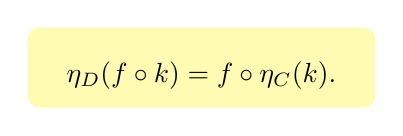
\begin{tikzpicture}
                    \filldraw[yellow!30, rounded corners] (-2.2, -0.4) rectangle (2.2,0.6);
                    \node at (0,0){$\eta_D(f \circ k)
                    =
                    f \circ \eta_C(k)$.};
                \end{tikzpicture}
            \end{tikzcd}
        \end{center}        
        We see that these functions must satisfy the 
        property outlined in yellow for all $C,D$. So 
        what functions do this?
        An immediate source of such functions that 
        assemble into natural transformations which we 
        seek arise when we take any $\phi \in \hom(B,A)$ and set 
        each $\eta_C : \hom(A,C) \to \hom(B,C)$ equal to 
        \[
            (-) \circ \phi : \hom(A,C) \to \hom(B,C)
        \]
        for each $C \in \cc$. This clearly checks out since we  
        have that, for any $f: C \to D$ and $k: A\to C$,  
        \[
            (f \circ k)\circ \phi = f  \circ (k \circ \phi).
        \]
        The question now is: Is every natural transformation 
        derived from some $\phi  \in  \hom(B,A)$? We know that the answer 
        is yes! This is an exercise in Section \ref{section:natural_transformations}. 
        The work of that exercise is proving this; however, 
        we  immediately get the  result 
        by the Yoneda Lemma since we can just observe that
        \[
            \text{Nat}(\hom(A, -), \hom(B, -))
            \cong
            \hom(B, A).   
        \]
        Therefore, each  such natural transformation is created from 
        some $\phi  \in  \hom(B,A)$,  which is what we'd expect,
        so the Yoneda lemma passes our sanity check.

    \end{example}

    We now introduce the following definition to ease our discussion. 
    \begin{definition}
        Let $\cc$ be a category. A functor of the form $F: \cc\op \to \textbf{Set}$ 
        is called a \textbf{presheaf}\footnote{The name ``presheaf'' is due to the 
        fact that this concept is a 
        precursor to the concept of a \emph{sheaf}, which is outside of our scope 
        for the moment. }. As a presheaf may be viewed as an element 
        of the functor category $\text{Fun}(\cc\op, \textbf{Set})$, we can define such a category 
        as the \textbf{category of presheaves over $\cc$}. 
    \end{definition}

    A natural source of presheaves is one which we are already familiar with. 
    Given any locally small category $\cc$, we can take any 
    object $A$ of $\cc$ to produce the functor 
    \[
        \hom_{\cc}(-, A): \cc\op \to \textbf{Set}.
    \]
    This process itself induces a functor known as the \emph{Yoneda embedding}.

    \begin{definition}
        Let $\cc$ be a locally small category. The \textbf{Yoneda embedding} on $\cc$ 
        is the functor $\bm{y}: \cc \to \text{Fun}(\cc\op, \textbf{Set})$ where 
        for each object $A$
        \[
            \bm{y}(A) = \hom_{\cc}(-, A): \cc\op \to \textbf{Set}.  
        \]
    \end{definition}
    The reason why this is called the Yoneda embedding is because of the functor's 
    relationship with the Yoneda embedding, which should become clear in proving the 
    following proposition. 

    \begin{proposition}
        The Yoneda embedding $\bm{y}: \cc \to \text{Fun}(\cc\op, \textbf{Set})$
        is a full and faithful functor.
    \end{proposition}
    The proof of this proposition is left as an exercise. However, the Yoneda 
    embedding arises naturally in many calculations within category. It is used 
    to prove the following important proposition. 

    \begin{proposition}
        Every small category $\cc$ is concrete. 
    \end{proposition}

    \begin{prf}
        Recall that a \emph{concrete category} $\cc$ is one which has a
        faithful functor $F: \cc \to \textbf{Set}$. To demonstrate this 
        for small categories, first define the functor 
        \[
            C: \text{Fun}(\cc\op, \textbf{Set}) \to \textbf{Set}
        \]
        where a presheaf $P: \cc\op \to \textbf{Set}$ is mapped as 
        \[
            (P: \cc\op \to \textbf{Set}) \mapsto \coprod_{A \in \text{Ob}(\cc)} P(A).
        \]
        Note that the indexing of the disjoint union is where we use locally smallness. 
        This functor is fully faithful (exercise). As it is fully faithful, and the Yoneda 
        embedding $\bm{y}: \cc \to \text{Fun}(\cc\op, \textbf{Set})$ is faithful, 
        the composite functor 
        \[
            C \circ \bm{y}: \cc \to \textbf{Set}
        \]
        must be faithful. Hence we see that $\cc$ is concrete. 
    \end{prf}
    
    Finally, we end this section with a curious connection to group theory. 
    It turns out that Yoneda's Lemma can actually be used in the proof of Cayley's Theorem.
    Sometimes this statement is taken too literally by others 
    and they think ``Yoneda's Lemma is a \emph{generalization} of 
    Cayley's Theorem'' but that is simply 
    not true, so the reader is warned to not believe someone when they hear that.
    Put simply, Yoneda's Lemma offers a bijection on sets which, with a little extra \emph{separate} 
    work, extends to an isomorphism of groups.

    \begin{proposition}(Cayley's Theorem.)
        Let $(G,  \cdot)$ be a group. Then $G$ is isomorphic to a subgroup of $\text{Perm}(G)$.
    \end{proposition}

    \begin{prf}
        Recall that a group $(G, \cdot)$ can be regarded as a category $\cc$; specifically, 
        we construct a category with one object $\bullet$ and set $\hom_{\cc}(\bullet, \bullet) = U(G)$, 
        where $U: \textbf{Grp} \to \textbf{Set}$ is the forgetful functor.
        For each $g \in G$, a morphism is represented as $f_g: \bullet \to \bullet$,
        and we have that $f_g \circ f_{g'} = f_{g'\cdot g}$.

        Now consider the functor $\hom_{\cc}(\bullet, -): \cc \to \textbf{Set}$. 
        Such a functor produces the following data:
        \begin{itemize}
            \item We have that $\hom_{\cc}(\bullet, \bullet) = U(G)$
            \item We also get a family of \emph{bijections} $\phi_g: U(G) \to U(G)$ such that $\phi_g \circ \phi_{g'} = \phi_{g'\cdot g}$.
        \end{itemize}
        In other words, the functor imposes an action of $G$ on its 
        underlying set of elements $U(G)$ in \textbf{Set}.
        Specifically, we may write $\phi_{g'}(g) = g' \cdot g$ for each $g \in G$.
        Now what's a natural transformation $\eta$ between two functors?
        \[
            \eta: \hom_{\cc}(\bullet, -) \to \hom_{\cc}(\bullet, -).
        \]
        Since there is only one object of $\cc$, a natural transformation is \emph{one} function 
        $\eta: U(G) \to U(G)$ such that for each $g'\in G$, 
        the diagram below commutes. 
        \begin{center}
            \begin{tikzcd}[column sep = 1.4cm, row sep = 1.4cm]
                \bullet
                \arrow[d, swap, "f_{g'}"]
                \\
                \bullet
            \end{tikzcd}
            \hspace{0.7cm}
            \begin{tikzcd}[column sep = 1.4cm, row sep = 1.4cm]
                U(G)
                \arrow[r, "\eta"]
                \arrow[d, swap, "\phi_{g'}"]
                &
                U(G)
                \arrow[d, "\phi_{g'}"]\\
                U(G)
                \arrow[r, swap, "\eta"]
                &
                U(G)
            \end{tikzcd}
            \hspace{0.7cm}
            \begin{tikzcd}[column sep = 1.4cm, row sep = 1.4cm]
                g
                \arrow[d, maps to]
                \arrow[r, maps to]
                &
                \eta(g)
                \arrow[d, maps to]
                \\  
                g' \cdot g
                \arrow[r, maps to]
                &
                \eta(g' \cdot g)
                = g' \cdot \eta(g)
            \end{tikzcd}
        \end{center}
        Now, Yoneda's Lemma gives us the bijection below, which we may denote as 
        $\psi$,
        \[
            \text{Nat}(\hom_{\cc}(\bullet, -), \hom_{\cc}(\bullet, -))
            \cong
            \hom_{\cc}(\bullet, \bullet) = U(G).
        \]
        If we now observe that 
        \begin{itemize}
            \item The collection of such natural transformations is a group under composition, with identity $1_{U(G)}: U(G) \to U(G)$,
            which we may denote as $(P, \circ)$
            \item $(P,  \circ) \subset \text{Perm}(G)$ 
        \end{itemize}
        then we can extend the isomorphism $\psi: P \to U(G)$ to a group isomorphism 
        \[
            \psi: (P, \circ) \isomarrow (G, \cdot) 
        \]
        which is the statement of Cayley's Theorem.
    \end{prf}

    {\large \textbf{Exercises}
    \vspace{0.5cm}}

    The first two exercises are very important. We (in fact you! The reader!) will 
    use these results later on. 

    \begin{itemize}
        \item[\textbf{1.}]\label{exercise:universality_bijection} 
        Prove the following dual counterpart to Proposition \ref{proposition:universality_bijection}: 
        Let $F: \cc \to \dd$ be a functor. Then a pair $(R, u: F(R) \to D)$ 
        is universal from \universalFToD{$F$ to $D$} if and only if for each $C \in \cc$, we have the 
        natural bijection 
        \[
            \hom_{\cc}(C, R) \cong \hom_{\dd}(F(C), D).
        \]

        \item[\textbf{2.}]\label{exercise:representable_if_and_only_if} 
        Prove the following dual counterpart to Proposition \ref{proposition:representable_if_and_only_if}:
        Let $\cc$ be a locally small category, and suppose $K: \cc \to \textbf{Set}$ 
        is a functor. Then $K$ is corepresentable, with representing object $R$, if and only if 
        $(R, u: K(R) \to \{\bullet\})$
        is universal from \universalFToD{$K$ to $\{\bullet\}$} for some object $R$. 

        \emph{Hint:} Because $K$ is corepresentable, it is a contravariant functor. Thus, this 
        should be very similar to the proof of Proposition \ref{proposition:representable_if_and_only_if}, 
        except with one twist.
    \end{itemize}

    \newpage
    \section{Finite Products}
    In this section we will discuss products in categories, which will be 
    our first  encounter with  the 
    concept of a \emph{limit}, something which has 
    yet to be defined. The concept of a limit, and the dual concept of a 
    colimit, form one of the central concepts of category theory. It will turn out that both 
    the limit and colimit concepts are a special case of a universal morphism.
    

    \begin{example}
        Let $(G, \textcolor{NavyBlue}{\bigcdot})$ and $(H, \textcolor{Orange}{\bigcdot})$
        be two groups with group operations $\textcolor{NavyBlue}{\bigcdot}: G \times G \to G $
        and $\textcolor{Orange}{\bigcdot}:  H \times H \to H$. The \textbf{product group} 
        of $G,H$ is the group 
        \[
            (G \times H, \bigcdot) = \bigg\{(g, h) \;\bigg|\; g \in G, \, h \in H \bigg\}
        \]
        whose group product works as 
        \[
            (g, h) \, \bigcdot \, (g', h') = (g \mathbin{\textcolor{NavyBlue}{\bigcdot}} g', h \mathbin{\textcolor{Orange}{\bigcdot}} h').
        \]
        One may check that this construction satisfies the definition of a group. 

        If $G, H$ are abelian groups, then the term ``group product'' is replaced 
        with the term \textbf{direct sum} (we will explain why later). In this case, the 
        product is denoted  $(G \oplus H, \bigcdot)$, and the group operation does not 
        change from above. 

        Direct sums, or more generally products of groups, are frequently used in group  
        theory. For example, they are necessary to describe the fundamental theorem 
        of finite abelian groups, which states that for any finite abelian group $A$, 
        there exist primes $p_1, p_2, \dots, p_n$ and positive integers $\alpha_1, \alpha_2, \dots, \alpha_n$ 
        such that 
        \[
            A \cong \zz_{p^{\alpha_1}_1}\oplus \zz_{p^{\alpha_2}_2} \oplus \cdots \oplus \zz_{p^{\alpha_n}_n}.
        \]
        That is, every finite abelian group is the product of cycic groups of a prime-power 
        order. 
    \end{example}

    \begin{example}        
        Let $(X, \tau_X)$ and $(Y, \tau_Y)$ be two topological spaces.
        Using $X$ and $Y$, we can create a topological space $(X \times Y, \tau_{X \times Y})$
        where $\tau_{X\times Y}$ is the \textbf{product topology}. There are many ways of 
        defining this topology, but in the finite case, we can write 
        $\tau_{X\times Y}$ as
        \[
            \tau_{X\times Y}  = \bigg\{ U \times V \;\bigg|\; U \in \tau_X, V \in \tau_Y \bigg\} . 
        \]
        In the way we have presented this, this is actually the \textbf{box topology}, but the 
        reader may recall that they coincide when we take finite products. 

    \end{example}

    \begin{example}
        In \textbf{Set}, we can always take two sets $X, Y$ to create  
        the \textbf{cartesian  product} $X \times Y$ defined as the set 
        \[
            X \times Y  =  \bigg\{ (x,y)  \;\bigg|\; x \in X, y \in Y \bigg\}
        \]
        Now consider the following question.
        \begin{center}
            \begin{minipage}{0.8\textwidth}
                \textbf{Q:}
                What 
                is the bare minimum amount of logical data that perfectly characterizes 
                the above product $X \times Y$?  
            \end{minipage}
        \end{center}
        Well, observe that for such a set, we have \emph{two} \textbf{projection 
        functions} 
        \begin{align*}
            &p_1: X \times Y \to X \qquad p_1(x, y) = x\\
            &p_2: X \times Y \to Y \qquad p_2(x, y) = y.
        \end{align*}
        Further, suppose that $f: Z \to X$ and $g: Z \to Y$ are two functions. 
        Then there exists a third $h: Z \to X \times Y$ such that $p_1\circ h = f$
        and $p_2\circ h = g$. By this description, we can deduce that 
        $h(z) = (f(z), g(z))$.
        \begin{align}\label{diagram:cartesian_product}
            \begin{tikzcd}[column sep = 1.4cm, row sep = 1.4cm
                ,ampersand replacement=\&]
                \&
                Z 
                \arrow[dr,  "g"]
                \arrow[dl, swap,"f"]
                \arrow[d, dashed, "h"]
                \&
                \\
                X 
                \& 
                \arrow[l, "p_1"]
                X \times Y 
                \arrow[r, swap, "p_2"]
                \&
                Y
            \end{tikzcd}
            \hspace{0.5cm}
            \begin{tikzcd}[column sep = 1.4cm, row sep = 1.4cm
                ,ampersand replacement=\&]
                \&
                z
                \arrow[dr, maps to]
                \arrow[dl, maps to]
                \arrow[d, maps to]
                \&
                \\
                f(z) 
                \& 
                \arrow[l, maps to]
                (f(z), g(z))
                \arrow[r, maps to]
                \&
                g(z)
            \end{tikzcd}
        \end{align}
        Moreover, this $h$ is \textbf{unique} with respect to $f$ and $g$; Showing this is the bulk of 
        Exercise \ref{section:universal_morphisms}.\exerciseCartesianProduct.
        We now have an answer to our question.

        \begin{center}
            \begin{minipage}{0.8\textwidth}
                \textbf{A:} The product $X \times Y$ is 
                characterized by the following data: two projection functions 
                $p_1: X\times Y \to X, p_2: X \times Y \to Y$, such that for any 
                pair of functions $f: Z \to X, g: Z \to Y$, there exists a \textbf{unique}
                third $h: Z \to X \times Y$ such that diagram \ref{diagram:cartesian_product} commutes.
            \end{minipage}
        \end{center}
    \end{example}

    With the above example in mind, we now introduce our first definition of a product.

    \begin{definition}[Nice Product Definition.]
        Let $\cc$ be a category with objects $A$ and $B$. 
        The \textbf{product of $A$ and $B$} is an object $A \times B$ 
        equipped with morphisms
        \[
            \pi_A: A \times B \to A \qquad 
            \pi_B: A \times B \to B            
        \]
        with the following universal property: For any object $Z$ of $\cc$ with morphisms
        $f: Z \to A$, $g: Z \to B$, there exists a unique morphism $h: Z \to A \times B$ 
        such that the diagram below commutes. 
        \begin{center}
            \begin{tikzcd}[column sep = 1.4cm, row sep = 1.4cm]
                &
                Z 
                \arrow[dr,  "g"]
                \arrow[dl, swap,"f"]
                \arrow[d, dashed, "h"]
                &
                \\
                A
                & 
                \arrow[l, "\pi_A"]
                A \times B
                \arrow[r, swap, "\pi_B"]
                &
                B
            \end{tikzcd}
        \end{center}
    \end{definition}

    \begin{remark}
        Note that to utilize the above universal property, one requires a \emph{pair} of morphisms 
        $f: Z \to A$ and $g: Z \to B$. That is, it is not true that, if I have a single 
        morphism $f: Z \to A$, then there exists a unique $h: Z \to A \times B$ such that $\pi_A \circ h = k$. 
        That would be false in many cases. 
    \end{remark}
    
    The above definition is a very nice one. For example, it returns the 
    concepts of products of groups or topological spaces when it is imposed 
    in \textbf{Grp} and \textbf{Top}. However, keep in mind the products don't 
    always exist. For example, it does not work in \textbf{Fld}, 
    the category of Fields (that is, there is no field which satisfies the universal property). 
    We will eventually explain why.

    \begin{example}
        Consider \textbf{Ring}, the category of rings. We can create products in this category 
        as follows: Let $(R, \mathbin{\textcolor{NavyBlue}{+}}, \mathbin{\textcolor{NavyBlue}{\bigcdot}})$
        and $(S, \mathbin{\textcolor{Orange}{+}}, \textcolor{Orange}{\bigcdot})$ be two rings 
        with zeros $0_R, 0_S$ and units $1_R, 1_S$. 
        Then we may form the \textbf{product ring} of $R$ and $S$ to be the ring 
        \[
            (R \times S, +, \bigcdot) = \bigg\{(r, s) \;\bigg| \; r \in R, s \in S \bigg\}
        \]
        where for all pairs $(r_1, s_1)$ and $(r_2, s_2)$ in $R \times S$, we define the ring operations to behave as
        \begin{itemize}
            \item $(r_1, s_1) + (r_2, s_2) = (r_1 \mathbin{\textcolor{NavyBlue}{+}} r_2, s_1 \mathbin{\textcolor{Orange}{+}} s_2)$ 
            \item $(r_1, s_1)\mathbin{\bigcdot} (r_2, s_2) = (r_1 \mathbin{\textcolor{NavyBlue}{\bigcdot}} r_2, s_1 \mathbin{\textcolor{Orange}{\bigcdot}} s_2)$
        \end{itemize}
        Note that with these requirements, the additive identity is $(0_R, 0_S)$ while the multiplicative identity 
        is $(1_R, 1_S)$. With this construction, one can show that this satisfies the universal property 
        of a product in \textbf{Ring}, so that \textbf{Ring} has products. 
    \end{example}

    We make an interesting observation from the last example. For our ring $(R \times S, +, \bigcdot)$, 
    we surely have that $(0_R, 1_S)$ and $(1_R, 0_R)$ are elements of the product ring. However, 
    \[
        (0_R, 1_S) \mathbin{\bigcdot} (1_R, 0_S) = (0_R \mathbin{\textcolor{NavyBlue}{\bigcdot}} 1_R, 0_S \mathbin{\textcolor{Orange}{\bigcdot}} 1_S)
        = 
        (0_R, 0_S).
    \]
    Hence, even if the rings $R$ and $S$ are integral domains, $R \times S$ is not an integral domain. 
    Thus the product of two rings is never an integral domain. 

    \begin{example}
        Consider the category of fields \textbf{Fld}. Let $F_1, F_2$ be fields. Then 
        we would expect that the ring 
        \[
            F_1 \times F_2 = \bigg\{ (a, b) \;\bigg|\; a \in F_1, F_2 \bigg\}
        \]
        to be the ``product field.'' But we just observed that this cannot 
        be a field because the product ring is not even an integral domain.

        However, this does not exclude the possibility that there is some kind of 
        other field construction which we are not considering that plays the role as 
        a product in \textbf{Fld}. We show that such a construction cannot 
        hold for all fields with the following simple example.

        Consider the fields $\mathbb{F}_2$ and $\mathbb{F}_3$, the fields with 2 and 3 elements, respectively. 
        Suppose that $P$ is the product field of 
        $\mathbb{F}_2$ and $\mathbb{F}_3$. Then by definition, we would require 
        two projection field homomorphisms
        \[
            \pi_1: P \to \mathbb{F}_2 \qquad \pi_2: P \to \mathbb{F}_3
        \]
        However, recall that two fields share a (nonzero) field homomorphism if and only if 
        they are of the same characteristic. Therefore, 
        \begin{itemize}
            \item $\pi_1$ can only exist if $P$ has characteristic 2. In fact, $P$ must be isomorphic to $\mathbb{F}_2$.
            \item $\pi_2$ can only exist if it has characteristic 3. In fact, $P$ must be isomorphic $\mathbb{F}_3$. 
        \end{itemize}
        Clearly, we have a contradiction.
        Thus we simply cannot generally take products in $\textbf{Fld}$ in a logical way.
    \end{example}

    

From the previous example, we see that products don't always exist in category. 
However, if they do, then we can take finitely many products. For instance, if we have 
three objects $A, B, C$, then we can take the products
\[
    A \times (B \times C) \qquad (A \times B) \times C.
\]
If we have four objects, then we can create 5 products. Thus, if we can take the 
product of two objects, then we all finite products consisting of objects of $\cc$ exist 
in our category.

We encapsulate this idea and include other prerequisites for a
category to have finite products in the following proposition. 

\begin{proposition}\label{prop_category_finite_products}
    Suppose $\cc$ is a category with a terminal object $T$ and a product
    object $A \times B$ for every pair of objects $A$ and $B$. Then 
    \begin{description}
        \item[$\bm{(i)}$] $\cc$ has finite products. 
        \item[$\bm{(ii)}$] There exists a bifunctor $\prod: \cc \times \cc
        \to \cc$ where $(A, B) \mapsto A \times B$.

        \item[$\bm{(iii)}$] For any three objects, we have an
        isomorphism 
        \[
            (A \times B) \times C \cong A \times (B \times C)
        \]
        which is natural in $A, B$ and $C$ .

        \item[$\bm{iv}$] For any object $A$, we have the isomorphism 
        \[
            T \times A \cong A \cong T \times A            
        \] 
        natural in $A$.
    \end{description}
\end{proposition}

\begin{prf}
    To prove the first part, let $P(n)$ be the following statement: 
    \[
        P(n) = 
        \begin{cases}
            \text{ For any objects } A_1, A_2, \dots, A_n \in \cc,\\
            \text{ their product diagram in }\cc.
        \end{cases}
    \]
    \begin{description}
        \item[Base Case.] Observe that for $n = 0$,  the statement is
        automatically true since we are given that a terminal object
        $T$ exists. 

        \item[Inductive Step.] Suppose the statement holds for $n =
        k$. Then for any objects $A_1, A_2, \cdots, A_k$, 
        we have the product diagram
        \begin{center}
            \begin{tikzcd}[column sep =  1.4cm, row sep = 1.4cm]
                & & D \arrow[d, dashed, "u"] 
                \arrow[ddll, bend right, swap, "f_1"]
                \arrow[ddl, bend right, crossing over, swap, "f_2"]
                \arrow[ddr, bend left, crossing over, "f_{k-1}"]
                \arrow[ddrr, bend left, "f_{k}"]
                & &  \\
                & & A_1  \times \cdots \times A_n 
                \arrow[dll, near start, swap, "\pi_1"]
                \arrow[dl, "\pi_2"] 
                \arrow[dr, swap, "\pi_{k-1}"]
                \arrow[drr, near start, "\pi_k"] & & \\
                A_1 & A_2 & \cdots & A_{k-1} & A_k
            \end{tikzcd}
        \end{center}
        and a unique, induced arrow $u$ whenever such a $D \in \cc$ with
        morphisms $f_i: D \to A_i$ exists.

        Let $A_{k+1}$ be an arbitrary object of $\cc$. Then the
        product $(A_1 \times A_2 \times \cdots \times A_k)\times
        A_{k+1}$ exists, since by assumption,  
        the product of any two objects in our
        category must exist, and gives rise to the product diagram: 
        \begin{center}
            \begin{tikzcd}[column sep =  1.4cm, row sep = 1.4cm]
                & D \arrow[d, dashed, "v"] 
                \arrow[dl, swap, end anchor={[xshift = -0.6cm]} , "g_1"] 
                \arrow[dr, "g_2"]
                & \\ 
                A_1 \times \cdots \times A_k 
                & 
                \arrow[l, "\pi'_1"] 
                A_1 \times \cdots \times A_k \times A_{k+1}
                \arrow[r, swap, "\pi'_2"]
                &
                A_{k+1}
            \end{tikzcd}
        \end{center}
        whenever such an object $D$ with a family of morphisms $g_1: D
        \to A_1 \times A_k$ and  $g_2: D \to A_{k+1}$ exist.

        Look at the bottom of the second diagram; we have a unique
        morphism $\pi'_1: A_1 \times \cdots \times A_k \times A_{k+1}
        \to A_1 \times \cdots \times A_k$.
        We can extend this across the morphisms $\pi_1, \pi_2 \cdots,
        \pi_k$ to demonstrate that there exist unique morphisms 
        \[
            \pi_i \circ \pi'_1: A_1 \times \cdots \times A_k \times A_{k+1}
            \to 
            A_i
        \]
        for $i = 1, 2, \dots, k$. Denote these as $\overline{\pi}_i$.
    
        Now suppose we there exists an object $C$ in $\cc$ with a
        family of morphisms $h_i: C \to A_i$. Then by the first
        diagram, there exists a unique morphism $u: C \to A_1 \times \cdots
        \times A_k$ such that $h_i = \pi_i \circ u$. Thus we have the
        diagram:
        \begin{center}
            \begin{tikzcd}[column sep =  1.4cm, row sep = 1.4cm]
                & C \arrow[d, dashed, "v"] 
                \arrow[dl, end anchor={[xshift = -0.6cm]}, swap, "u"] 
                \arrow[dr, "h_{k+1}"]
                & \\ 
                A_1 \times \cdots \times A_k 
                & 
                \arrow[l, "\pi'_1"] 
                A_1 \times \cdots \times A_k \times A_{k+1}
                \arrow[r, swap, "\pi'_2"]
                &
                A_{k+1}
            \end{tikzcd}
        \end{center}    
        so we have a unique morphism $v: C \to A_1 \times \cdots
        \times A_{k+1}$ such that $\pi'_1 \circ v = u$ and $\pi'_2
        \circ v = h_{k+1}$. 
        However, note that 
        \[
            \pi'_1 \circ  v = u \implies (\pi_i \circ \pi'_1) \circ v = 
            \pi_i \circ u 
            \implies \overline{\pi}_i \circ v= h_i.
        \]
        for $i = 1, 2, \dots, k$. 
        
        Now let $\overline{\pi}_{k+1} =
        \pi'_2$. 
        Then we see that for such a family $h_i: C \to A_i$ for $i =
        1,  2, \dots, k+1$, there exists a unique morphism $v: C \to
        A_1 \times \cdots \times A_{k+1}$ such that 
        \[
            \overline{\pi}_i \circ v = h_i
        \]
        for $i = 1, 2, \dots, k + 1$. Therefore, we have the product
        diagram 
        \begin{center}
            \begin{tikzcd}[column sep =  1.4cm, row sep = 1.4cm]
                & & C \arrow[d, dashed, "v"] 
                \arrow[ddll, bend right, swap, "h_1"]
                \arrow[ddl, bend right, crossing over, swap, "h_2"]
                \arrow[ddr, bend left, crossing over, "h_{k}"]
                \arrow[ddrr, bend left, "h_{k+1}"]
                & &  \\
                & & A_1  \times \cdots \times A_{k+1} 
                \arrow[dll, near start, swap, "\overline{\pi}_1"]
                \arrow[dl, "\overline{\pi}_2"] 
                \arrow[dr, swap, "\overline{\pi}_{k}"]
                \arrow[drr, near start, "\overline{\pi}_{k+1}"] & & \\
                A_1 & A_2 & \cdots & A_{k} & A_{k+1}
            \end{tikzcd}
        \end{center}
        so that the product $A_1 \times A_k \times A_{k+1}$ exists and
        is well-defined in $\cc$. Hence, $P(n)$ is true for $n = k+1$.
    \end{description}
    By mathematical induction, we see that all finite products must
    exist in $\cc$, as desired. 

    To demonstrate the existence of a bifunctor, we can directly
    define one. Let $\prod: \cc \times \cc \to \cc$ act as follows. 
    \begin{description}
        \item[Objects.] $\prod(A, B) = A \times B$.
        \item[Morphisms.] Let $f: A \to A'$ and $g: B \to B'$. Suppose
        we have canonical projections 
        \[
            \pi_1: A \times B \to A \qquad  \pi_2: A \times B \to B  
        \] 
        and 
        \[
            \pi'_1: A' \times B' \to A' \qquad  \pi'_2: A' \times B' \to  
            B'.
        \]
        Then observe we get the diagram
        \begin{center}
            \begin{tikzcd}[column sep =  1.4cm, row sep = 1.4cm]
                & A \times B \arrow[d, dashed, "u"] 
                \arrow[dl, swap, "f \circ \pi_1"] 
                \arrow[dr, "g \circ \pi_2"]
                & \\ 
                A'
                & 
                \arrow[l, "\pi'_1"] 
                A' \times B'
                \arrow[r, swap, "\pi'_2"]
                &
                B'
            \end{tikzcd}
        \end{center}
        Thus, there exists a unique morphism $u: A \times B \to A'
        \times B'$ whenever such $f, g$ exist. Therefore, we can
        define how $\prod$ acts on morphism as
        \[
            \prod(f: A \to A', g: B \to B') = u: A \times B \to A' \times
            B'
        \]
        where $u$ is generated by the diagram above. As we just showed, 
        this assignment is well-defined.
        It's now pretty straightforward to now show that this establishes
        a functor (and I'm too lazy to do so). 

        To establish associativity of our products, we demonstrate
        they're  isomorphic. Thus let $A \times (B \times C)$ and $(A
        \times B) \times C$ be two products in $\cc$. Suppose we have
        an family of morphisms $h_1: D \to A$, $h_2: D \to B$ and
        $h_3: D \to C$. Then we get the following product diagrams. 

        \begin{minipage}{0.5\textwidth}
            \begin{center}
                \begin{tikzcd}[column sep =  1.4cm, row sep = 1.4cm]
                    & D \arrow[d, dashed, Blue, "v"] 
                    \arrow[dl, swap, "h_2"] 
                    \arrow[dr, "h_3"]
                    & \\ 
                    B
                    & 
                    \arrow[l, "p_1"] 
                    B \times C
                    \arrow[r, swap, "p_2"]
                    &
                    C
                \end{tikzcd}
                \hspace{1cm}
                \begin{tikzcd}[column sep =  1.4cm, row sep = 1.4cm]
                    & D \arrow[d, dashed, Red, "w"] 
                    \arrow[dl, swap, "h_1"] 
                    \arrow[dr, "h_2"]
                    & \\ 
                    A
                    & 
                    \arrow[l, "p'_1"] 
                    A \times B
                    \arrow[r, swap, "p'_2"]
                    &
                    B
                \end{tikzcd}
            \end{center}
        \end{minipage}
        \begin{minipage}{0.5\textwidth}
            \begin{center}
                \begin{tikzcd}[column sep =  1.4cm, row sep = 1.4cm]
                    & & D \arrow[d, dashed, "u"]
                    \arrow[ddl, swap, bend right = 45, "h_1"]
                    \arrow[dd, near start, swap, bend right = 50, "h_2"]
                    \arrow[ddr, bend left = 45, "h_3"]
                    & &\\
                    & & A \times B \times C 
                    \arrow[dl, swap, "\overline{\pi}_1"] 
                    \arrow[d, "\overline{\pi}_2"] 
                    \arrow[dr, "\overline{\pi}_3"]& & \\
                    & A & B & C &
                \end{tikzcd}
            \end{center}
        \end{minipage}
        Since we have unique morphisms $v: D \to B \times C$ and $w: D
        \to A \times B$, we also get the product diagrams. 
        \begin{center}
            \begin{tikzcd}[column sep =  1.4cm, row sep = 1.4cm]
                & D \arrow[d, dashed, "y"] 
                \arrow[dl, swap, "h_1"] 
                \arrow[dr, Blue, "v"]
                & \\ 
                A
                & 
                \arrow[l, "\pi_1"] 
                A \times (B \times C)
                \arrow[r, swap, "\pi_2"]
                &
                B \times C
            \end{tikzcd}
            \begin{tikzcd}[column sep =  1.4cm, row sep = 1.4cm]
                & D \arrow[d, dashed, "z"] 
                \arrow[dl, swap, Red, "w"] 
                \arrow[dr, "h_3"]
                & \\ 
                A \times B
                & 
                \arrow[l, "\pi'_1"] 
                (A \times B) \times C
                \arrow[r, swap, "\pi'_2"]
                &
                C
            \end{tikzcd}
        \end{center}
        for the products $A \times (B \times C)$ and $(A \times B)
        \times C$, respectively. Thus we have the collection of
        morphisms 
        \begin{align*}
            &p_1' \circ \pi'_1 : (A \times B) \times C \to A \quad 
            &&\pi_1: A \times (B \times C) \to A\\
            &p_2' \circ \pi'_1 : (A \times B) \times C \to B \quad 
            &&p_1 \circ \pi_2: A \times (B \times C) \to B\\
            &\pi'_2 : (A \times B) \times C \to C \quad 
            &&p_2 \circ \pi_2: A \times (B \times C) \to C.
        \end{align*}
        Now observe that 
        \begin{align}
            &p_1' \circ \pi'_1 \circ z = p'_1 \circ w = h_1 
            \quad 
            &&\pi_1 \circ y = h_1
            \\ 
            &p'_2 \circ \pi'_1 \circ x = p'_2 \circ w = h_2 
            \quad 
            &&p_1 \circ \pi_2 \circ y = p_1 \circ v = h_2
            \\
            &\pi'_2 \circ z = h_3 
            \quad 
            &&p_2 \circ \pi_2 \circ y = p_2 \circ v = h_3.
        \end{align}
        Thus we see that our  first collection of morphisms are 
        projections. That is, for any family of morphisms $h_1: D \to
        A$, $h_2: D \to B$ and $h_3: D \to C$, there exists unique
        morphisms such that equations $y, z$ such that equations (3),
        (4) and (5) hold. 
        What this means is that $A \times  (B \times C)$ and $(A
        \times B) \times C$ are universal objects; specifically, they
        form universal cones. However, the original 
        universal cone of this construction was simply $A \times B 
        \times C$ with the morphisms $\overline{\pi}_1,
        \overline{\pi}_2, \overline{\pi}_3$. Thus we have that
        \[
            A \times (B \times C) \cong (A \times B) \times C \cong A 
            \times B \times C
        \]
        since universal objects of the same construction are
        isomorphic. Showing naturality is not hard (again, too lazy to
        do that).
        
        Finally, let $T$ be the terminal object of $\cc$. Denote $t_C:
        C \to T$ as the unique morphism from $C$ to $T$. Now consider
        the product diagram associated with the product $T \times A$: 
        \begin{center}
            \begin{tikzcd}[column sep =  1.4cm, row sep = 1.4cm]
                & D \arrow[d, dashed, "u"] 
                \arrow[dl, swap, "t_D"] 
                \arrow[dr, "f"]
                & \\ 
                T
                & 
                \arrow[l, "t_A"] 
                T \times A
                \arrow[r, swap, "\pi"]
                &
                A
            \end{tikzcd}
        \end{center}
        Observe that $t_D$ always exists for any $D$. Hence the
        existence of  $u$ is completely dependent $f$. Therefore, we
        can see that this diagram is equivalent  to 
        \begin{center}
            \begin{tikzcd}[column sep =  1.4cm, row sep = 1.4cm]
                & D \arrow[d, dashed, "u"] 
                \arrow[dl, swap, "t_D"] 
                \arrow[dr, "f"]
                & \\ 
                T
                & 
                \arrow[l, "t_A"] 
                A
                \arrow[r, swap, "1_A"]
                &
                A
            \end{tikzcd}
        \end{center}
        Hence we see that $A$ with the morphism $t_A, 1_A$ forms a
        universal cone. But so does $T \times A$; hence, uniqueness
        guarantees they are isomorphic. 
    \end{description}
\end{prf}

Now that we have discussed examples of products in categories, offered a rigorous definition, 
and we observed an example when they do not exist, we would naturally want to generalize 
this concept since it is often the case that we would like to take arbitrary products, or even 
infinite products. We also want to somehow connect products to a universal morphism. To do all 
of these things requires us to further abstract our definition of a product. 
Before doing so, we offer a simple definition.

\begin{definition}
    Let $\cc$ be a category.
    Define the \textbf{diagonal functor of $\cc$} as 
    $\Delta: \cc \to \cc \times \cc$ where 
    \begin{description}
        \item[On Objects.] For $C$ an object of $\cc$, we define $\Delta(C) = (C, C)$.
        \item[On Morphisms.] For a morphism $f: A \to B$, we define
        $\Delta(f) = (f, f): (A, A) \to (B, B)$.
    \end{description}
\end{definition}

The above functor is a bit silly; it really doesn't do much. However, it necessary for us 
to really understand what exactly a product is. It helps us realize that a product in 
a category is actually a universal morphism. 

\begin{definition}[Rigorous Product Definition.]
    Let $\cc$ be a category with objects $A, B$. The \textbf{product $A \times B$ of $A$ and $B$}
    is a universal morphism 
    \[
        \pi: (A \times B, u: \Delta(A\times B) \to (A, B))  
    \]
    from \hyperref[definition:universal_morphism_from_F_to_D]{\textcolor{blue}{$\Delta$ to $(A, B)$}}. This means that for any
    other pair $(C, q: \Delta(C) \to (A, B))$, there exists a unique 
    $h: C \to A \times B$ in $\cc$ such that the diagram below commutes. 
    \begin{center}
        \begin{tikzcd}[column sep = 1.4cm, row sep = 1.4cm]
            \Delta(A \times B)
            \arrow[r, "\pi"]
            &
            (A, B)
            \\
            \Delta(C)
            \arrow[u, dashed, "\Delta(h)"]
            \arrow[ur, swap, "q"]
            &
        \end{tikzcd}
    \end{center}
\end{definition}

This definition is exactly equivalent to our previous. What this tells us is that 
a product is an instance of a universal morphism. We show how this definition is equivalent 
to the previous via the following example.

\begin{example}
    To see this for the case when $n = 2$,
    consider the product $A\times B$ of two objects $A, B$ in some category $\cc$. 
    Then 
    \begin{center}
        \begin{tikzcd}[column sep = 1.4cm, row sep = 1.4cm]
            (A, B)
            &
            \Delta(A \times B) \arrow[l, swap, "u"]\\
            & \Delta(C) \arrow[u, swap, dashed, "\Delta(f')"]
            \arrow[ul, "h"]
        \end{tikzcd}
        =
        \begin{tikzcd}[column sep = 1.4cm, row sep = 1.4cm]
            (A, B)
            &
            (A \times B, A \times B) \arrow[l, swap, "{(\pi_A, \pi_B)}"]\\
            & (C, C) \arrow[u, dashed, swap, "{(f', f')}"]
            \arrow[ul, "h"]
        \end{tikzcd}
        \hspace{1cm}
        \begin{tikzcd}[column sep = 1.4cm, row sep = 1.4cm]
            A \times B\\
            C \arrow[u, dashed, "f'"]
        \end{tikzcd}
    \end{center}

    Let's spell out what's going on above; you might have seen this exposition, without even realizing, demonstrating the universality of
    products. Suppose there exists another object $C$ with morphisms
    $f: C \to A$ and $g: C \to B$. Then we force the existence of a
    morphism $f': C \to A \times B$.
    \begin{center}
        \begin{tikzcd}[column sep = 1.4cm, row sep = 1.4cm]
            A 
            & \arrow[l, swap, "\pi_A"] A \times B \arrow[r, "\pi_B"] 
            & 
            B \\
            & \arrow[ul, "f"] C \arrow[u, dashed, "f'"] \arrow[ur, swap, 
            "g"]&
        \end{tikzcd}
    \end{center}
    When we usually do this, we simply just set 
    \[
        f' = (f, g)   
    \]
    so that $\pi_A \circ f' = f$, and $\pi_B \circ f' = g$. 
\end{example}


\newpage
\section{Finite Coproducts}

We now move onto the concept of coproducts in categories. We will see that this concept 
is an instance of a \emph{colimit}, which is yet to be defined. We build intuition 
on the concept with the special concept of coproducts by introducing examples. 

\begin{example}\label{example:free_product}
    Let $(G, \textcolor{NavyBlue}{\bigcdot})$ and $(H, \textcolor{Orange}{\bigcdot})$
    be two groups with group operations $\textcolor{NavyBlue}{\bigcdot}: G \times G \to G $
    and $\textcolor{Orange}{\bigcdot}:  H \times H \to H$. The 
    \textbf{free product} of $G$ and $H$ is the group 
    \[
        (G \* H, \bigcdot) = \bigg\{ g_1h_1g_2h_2\cdots g_kh_k \;\bigg|\; g_i \in G, h_i \in H \bigg\}
    \] 
    with the following operation. If $g_1h_1\cdots g_kh_k$ and $g'_1h'_1\cdots g'_{\ell}h'_{\ell}$
    are two elements of $G \* H$, then 
    \[
        (g_1h_1\cdots g_kh_k) \mathbin{\bigcdot} (g'_1h'_1\cdots g'_{\ell } h'_{\ell } )
        = 
        g_1h_1\cdots g_kh_k g'_1h'_1 \cdots g'_{\ell}h'_{\ell}.
    \]
    We require the group operation to obey the following two rules. Let $g_1h_1\cdots g_kh_k \in G \* H$.
    \begin{itemize}
        \item If $g \in G$, then 
        \[
            g \mathbin{\bigcdot} (g_1h_1\cdots g_kh_k) = (g \mathbin{\textcolor{NavyBlue}{\bigcdot}} g_1)h_1\cdots g_kh_k.
        \]
        \item If $h \in H$, then 
        \[
            (g_1h_1\cdots g_kh_k)\mathbin{\bigcdot} h = g_1h_1\cdots g_k(h_k \mathbin{\textcolor{Orange}{\bigcdot}} h).
        \]
    \end{itemize}
    The free product of two groups arise frequently in algebraic topology.
    Despite that its definition is somewhat complicated, we will see later
    that free products are in some sense dual to the concept of the product of groups. 
    The reader will also soon see that the naming ``free product'' is an unfortunate one 
    as it is somewhat misleading.

    Free products appear prominently in various statements of Van Kampen's theorem in topology; what 
    follows is a simplified version.
    If $X = U \cup V$ is a topological space with $U, V$ open sets, and 
    if $U \cap V \ne \varnothing$ is path connected and simply connected, then 
    \[
        \pi_1(X) \cong \pi_1(U)\* \pi_1(V)
    \]
    where $\pi_1(X)$ is the fundamental group of $X$. (Note that since $X$ is path connected, 
    it doesn't matter what basepoint for the fundamental group we select). 
    % Cite Page 177 of Topology Through Inquiry. 
\end{example}

We will soon see that the free product is the coproduct in the category of \textbf{Grp}, although 
such a statement should not make any sense the reader until we define what a coproduct is. 

\begin{example}
    In \textbf{Set}, we can combine two different sets $X$ and $Y$ to create the 
    \textbf{disjoint union} $X \amalg Y$, which is defined to be the set 
    \[
        X \amalg Y = \bigg\{ (x, 0), (y, 1) \;\bigg|\;  x \in X, y \in Y  \bigg\}.
    \]
    In the above set, elements are tuples whos first coordinate is either 
    in $X$ or $Y$, and the second is some value which depends on whether or not the first 
    coordinate is in $X$ or $Y$. 
    I decided to make these values 0 and 1, but it is ultimately arbitrary. 
    We just need to make sure that these values are distinct so that we can determine if a tuple 
    has an element from $X$ or $Y$ based on the value in the second slot. For example, for a tuple $(z, 0)$, 
    we know that $z \in X$. If the tuple is of the form $(z, 1)$, we know that $z \in Y$. 

    We perform a similar analysis as before with products, and we consider the following question.
    \begin{center}
        \begin{minipage}{0.8\textwidth}
            \textbf{Q:}
            What 
            is the bare minimum amount of logical data that perfectly characterizes 
            the above disjoint union $X \amalg Y$?  
        \end{minipage}
    \end{center}

    Observe that we have the two \textbf{inclusion functions}
    \begin{align*}
        &i_1: X \to X \amalg Y \qquad i_1(x) = (x, 0)\\
        &i_2: Y \to X \amalg Y \qquad i_2(y) = (y, 1).
    \end{align*}
    These two functions are equipped with the following remarkable property. 
    Let $Z$ be some set, and suppose I have two functions
    \begin{align*}
        &f: X \to X \amalg Y \\
        &g: Y \to X \amalg Y.
    \end{align*}
    Then there exists a unique function $h: X \amalg Y \to Z$ such that the diagram below 
    commutes. 
    \begin{align}\label{diagram:disjoint_union_diagram}
        \begin{tikzcd}[column sep = 1.4cm, row sep = 1.4cm
            ,ampersand replacement=\&]
            \&
            Z 
            \arrow[<-, dr,  "g"]
            \arrow[<-, dl, swap,"f"]
            \arrow[<-, d, dashed, "h"]
            \&
            \\
            X 
            \& 
            \arrow[<-, l, "i_1"]
            X \amalg Y 
            \arrow[<-, r, swap, "i_2"]
            \&
            Y
        \end{tikzcd}
        \qquad
        h(z, i)
        =
        \begin{cases}
            f(z) & \text{if } i = 0\\ 
            g(z) & \text{if } i = 1
        \end{cases}
    \end{align}
    This definition of this unique $h: X \amalg Y \to Z$ is described above on the right.
    With the above definition, one can easily see that the above diagram does in fact commute.
    We now have an answer to our question.
    \begin{center}
        \begin{minipage}{0.8\textwidth}
            \textbf{A:} The disjoint union $X \amalg Y$ is characterized by two 
            inclusion functions $i_1: X \to X \amalg Y$, $i_2: Y \to X \amalg Y$, 
            such that, for any $f: X \to Z$, $g: Y \to Z$, there exists a \textbf{unique} 
            $h: X \amalg Y \to Z$ such that diagram \ref{diagram:disjoint_union_diagram} 
            commutes.
        \end{minipage}
    \end{center}
\end{example}

This now motivates the following definition of a \emph{coproduct}. 

\begin{definition}[Nice Coproduct Definition.]
    Let $\cc$ be a category with objects $A$ and $B$. The \textbf{coproduct} of $A$ and $B$ 
    is an object $A \amalg B$ of $\cc$ which is equipped with morphisms 
    \[
        i_A: A \to A \amalg B \qquad i_B: B \to A \amalg B
    \]
    with the following universal property: For any object $Z$ of $\cc$ with a pair 
    of morphisms $f: A \to Z$ and $g: B \to Z$, then there exists a unique morphism 
    $h: A \amalg B \to Z$ such that the diagram below commutes. 
    \begin{center}
        \begin{tikzcd}[column sep = 1.4cm, row sep = 1.4cm
            ,ampersand replacement=\&]
            \&
            Z 
            \arrow[<-, dr,  "g"]
            \arrow[<-, dl, swap,"f"]
            \arrow[<-, d, dashed, "h"]
            \&
            \\
            A 
            \& 
            \arrow[<-, l, "i_A"]
            A \amalg B 
            \arrow[<-, r, swap, "i_B"]
            \&
            B
        \end{tikzcd}
    \end{center}
\end{definition}

It is now clear that, coproducts in \textbf{Set} exist; it is the disjoint union.

\begin{remark}
    Note that to utilize the above universal property, one requires a \emph{pair} of morphisms 
    $f: A \to Z$ and $g: B \to Z$. That is, it is not true that, if I have a single 
    morphism $k: A \to Z$, then there exists a unique $h: A \amalg B \to Z$ such that $h \circ i_X = k$. 
    That would be false in many cases. 
\end{remark}

\begin{proposition}
    Suppose $\cc$ is a category with an initial object $I$ and a coproduct
    object $A \amalg B$ for every pair of objects $A$ and $B$. Then 
    \begin{description}
        \item[$\bm{(i)}$] $\cc$ has finite coproducts. 
        \item[$\bm{(ii)}$] There exists a bifunctor $\amalg: \cc \times \cc
        \to \cc$ where $(A, B) \mapsto A \amalg B$.

        \item[$\bm{(iii)}$] For any three objects, we have an
        isomorphism 
        \[
            (A \amalg B) \amalg C \cong A \amalg (B \amalg C) \cong A 
            \amalg B \amalg C
        \]
        which is natural in $A, B$ and $C$ .

        \item[$\bm{iv}$] For any object $A$, we have the isomorphism 
        \[
            I \amalg A \cong A \cong I \amalg A            
        \] 
        natural in $A$, where $T$ is the initial object of the category.
    \end{description}
\end{proposition}

\begin{definition}[Rigorous Coproduct Definition]
    Let $\cc$ be a category with objects $A, B$. The 
    \textbf{coproduct $A \amalg B$ of $A$ and $B$} is 
    a universal morphism 
    \[
        (A \amalg B, i: (A,B) \to \Delta(A \amalg B))
    \]
    from \hyperref[definition:universal_morphism_from_F_to_D]{\textcolor{blue}{$(A,B)$ to $\Delta$}}. 
    This means that, for any other pair $(C, j: (A, B) \to \Delta(C))$, there exists 
    a unique $h: A \amalg B \to C$ such that the diagram below commutes. 
    \begin{center}
        \begin{tikzcd}[column sep = 1.4cm, row sep = 1.4cm]
            (A, B) 
            \arrow[r, "i"]
            \arrow[dr, swap, "j"]
            &
            \Delta(A \amalg B)
            \arrow[d, dashed, "\Delta(h)"]
            \\
            &
            \Delta(C)
        \end{tikzcd}
        \hspace{1cm}
        \begin{tikzcd}[column sep = 1.4cm, row sep = 1.4cm]
            A \amalg B
            \arrow[d, dashed, "h"]
            \\
            C
        \end{tikzcd}
    \end{center}

    Visually, we have that 
    \begin{center}
    \begin{tikzcd}[column sep = 1.4cm, row sep = 1.4cm]
        (A, B) \arrow[r, "u"] \arrow[dr, swap, "f"] 
        & (C, C) \arrow[d, dashed, "{(h, h)}"]\\
        & (D, D)
    \end{tikzcd}
    \hspace{1cm}
    \begin{tikzcd}[row sep = 1.4cm]
        C \arrow[d, dashed, "h"]
        \\ 
        D
    \end{tikzcd}
    \end{center}
\end{definition}

    \newpage
    \section{Arbitrary Products and Coproducts in Categories}

    In this section, we perform a construction that allows us to have finite products and coproducts 
    in a category. Once we achieve that construction, we easily generalize our work 
    to obtain a definition for arbitrary products and coproducts in a category.
    \begin{definition}
    Let $\mathcal{D}_n$ be the discrete category with $n$-many objects (we use the letter $\dd$ for ``discrete''). 
    We will often visualize $\mathcal{D}_n$ as below.  
    \begin{align_topbot}
        \begin{tikzpicture}
            \filldraw[yellow!30, rounded corners] (-4.3, -0.7) rectangle (4.3,0.7);
            \node at (0,0){
                \begin{tikzcd}[ampersand replacement= \&]
                    \bullet_1 \arrow[out=120,in=60,looseness=3,loop]
                    \&
                    \bullet_2 \arrow[out=120,in=60,looseness=3,loop]
                    \&
                    \bullet_3 \arrow[out=120,in=60,looseness=3,loop]
                    \&
                    \cdots 
                    \& 
                    \bullet_n \arrow[scale = 1, out=123,in=57,looseness = 3, loop]
                \end{tikzcd}
            };
        \end{tikzpicture}
    \end{align_topbot}
    Note that 
    a functor $F: \dd_n \to \cc$ is one which simply picks out $n$ different objects $A_1$, $A_2, 
    \dots$, $A_n$ of $\cc$:
    \[
        F(\bullet_1) = A_1, \quad F(\bullet_2) = A_2, \quad  \dots,
        \quad
        F(\bullet_n) = A_n.
    \]
    This category allows us to make the following definition. 

    \begin{definition}
        Let $\cc$ be a category.
        The $n$-th \textbf{diagonal functor} $\Delta_n: \cc \to \cc^{n}$,
        is the functor defined as follows. 
        \begin{description}
            \item[On Objects.] For an object $C$, we have that $\Delta_n(C) = (\overbrace{C, C, \dots, C}^{n\text{-many copies}})$.
            \item[On Morphisms.] For a morphism $f: A \to B$ in $\cc$, we have that  
            \[
                \Delta_n(f: A \to B) = (f, f, \dots, f): \Delta_n(A) \to \Delta_n(B).
            \]    
        \end{description}
    \end{definition}
    The diagonal  functor is also sometimes informally called the 
    ``copy'' functor, since it is literally just copying data. We now 
    make some observations. 

    \begin{itemize}
        \item[(\textbf{1})] For each object $C \in \cc$, 
        we can interpret the object $\Delta_n(C) \in \cc^n$ 
        \emph{as a functor}
        \[
            \Delta_n(C): \mathcal{D}_n \to \cc
        \]
        where $\Delta_n(C)$ sends $\bullet_i$ to  $C$ for all $i= 1, 2, \dots, n$.

        \item[(\textbf{2})] Thus, we may also regard the $n$-th diagonal functor as a functor as below.
        \[
            \Delta_n: \cc \to \text{Fun}(\mathcal{D}_n, \cc) \qquad C \mapsto (\Delta_n(C) :\mathcal{D}_n \to \cc).
        \]
        In this interpretation, every morphism $f:C \to C'$ is interpreted as a natural 
        transformation $\Delta_n(f): \Delta_n(C) \to \Delta_n(C')$. 

        \item[(\textbf{3})] Consider a functor $F: \dd_n \to \cc$ such that $F(\bullet_i) = A_i \in \cc$. 
        For each $C \in \cc$, a natural transformation 
        \[
            \eta: \Delta_n(C) \to F
        \]
        will simply correspond to $n$-many morphisms $\eta_1, \dots, 
        \eta_n$ where
        \[
            \eta_i: \Delta_n(C)(\bullet_i) \to  F(\bullet_i) 
            \implies 
            \eta_i: C \to A_i.
        \]
    \end{itemize}
    \end{definition}
    With this notation clarified, we now can propose  our  definition of a  product. 

    \begin{definition}[Finite Product and Coproduct Definition]\label{definition:finite_products_and_coproducts}
    Let $\cc$ be a category. Let $A_1$, $A_2, \dots$, $A_n$ be objects of $\cc$. Let 
    $F: \mathcal{D}_n \to \cc$ be the functor such that $F(\bullet_i) = A_i$.
    
    \begin{itemize}
        \item The \textbf{product} of $A_1, A_2, \dots, A_n$ 
        is an object $P$ of $\cc$ equipped with
        a (natural transformation) $ \displaystyle p: \Delta_n\left( P \right) \to F$ 
        such that 
        \begin{center}
            $\displaystyle \left( P, p: \Delta_n\left( P \right) \to F \right)$
            is universal from 
            \hyperref[definition:universal_morphism_from_D_to_F]{\textcolor{blue}{$\Delta_n$ to $P$}.}
        \end{center}
        In the case where the product $P$ exists, we write $P = \prod_{i = 1}^{n} A_i$. 

        \item The \textbf{coproduct} of $A_1, A_2, \dots, A_n$
        is an object $C$ of $\cc$ equipped with 
        a (natural transformation) $i: F \to \Delta_n(C)$ such that 
            \begin{center}
                $(C, i: F \to \Delta_n(C))$ is universal from \hyperref[definition:universal_morphism_from_F_to_D]{\textcolor{blue}{$C$ to $\Delta_n$}}.
            \end{center}
        In the case where the coproduct $C$ exists, we write $C = \coprod_{i = 1}^{n} A_i$ 
        \end{itemize}

    \end{definition}
    \begin{remark}
        By Observation (\textbf{3}) as above, if $\displaystyle p: \Delta_n\left( \prod_{i=1}^{n}A_i \right) \to F$
        is a natural transformation, then it corresponds to $n$-many morphisms 
        \[
            p_k: \prod_{i=1}^{n}A_i \to A_k \qquad k = 1, 2, \dots, n
        \]
        This matches our intuition: A product of $n$-objects should always have 
        $n$-many morphisms between the product and each of its factors. 

        Similarly, a natural transformation $i: F \to \Delta_n\left( \coprod_{i = 1}^{n}A_i \right)$ corresponds to 
        $n$-many morphisms 
        \[
            i_k: A_k \to \coprod_{i = 1}^{n}A_i \qquad k = 1, 2, \dots, n
        \]
        which again matches our intuition: A coproduct of $n$-objects should have 
        $n$-many morphisms between each of its factors and the coproduct.
    \end{remark}
    
    We now have everything we need to define arbitrary products and coproducts, including 
    infinite ones.
    We just need to specify some notation that we will use.
    Towards that goal, let $\lambda$ be some indexing set.  
    \begin{itemize}
        \item Define $\dd_{\lambda}$ to be the discrete category consisting of one object $\bullet_i$ for each $i \in 
        \lambda$. (In particular, $\dd_{\lambda}$ is now possibly infinite.)
        \item Define the $\lambda$-diagonal functor to be the functor $\Delta_{\lambda}: \cc \to \text{Fun}(\dd_{\lambda}, \cc)$
        where $\Delta_{\lambda}(C): \dd_{\lambda} \to \cc$ 
        sends each $\bullet_i$ to $C$ for all $i \in \lambda$.
    \end{itemize}

    \begin{definition}[Arbitrary Product and Coproduct Definition]\label{definition:infinite_products_and_coproducts}
        Let $\cc$ be a category, and consider an arbitrary set of objects $\{A_i\}_{i \in \lambda}$ of $\cc$, $\lambda$ some indexing set.
        Let $F: \dd_{\lambda} \to \cc$ be the functor such that $F(\bullet_{i}) = A_i$ for $i \in \lambda$.

        \begin{itemize}
            \item The \textbf{product} of $\{A_i\}_{i \in \lambda}$ is the object 
            $P$ of $\cc$
            equipped with a (natural transformation) $\displaystyle p: \Delta_{\lambda}\left( P\right) \to F$ 
            such that 
            \begin{center}
                $\left( P, \Delta_{\lambda}\left( P \right) \to F \right)$ is universal from 
                \hyperref[definition:universal_morphism_from_F_to_D]{\textcolor{blue}{$\Delta_{\lambda}$ to $P$}.}
            \end{center}
            In the case where the product $P$ exists, we write $P = \prod_{i \in \lambda}A_i.$

            \item The \textbf{coproduct} of $\{A_i\}_{i \in \lambda}$ is the object 
            $C$ of $\cc$ equipped with a (natural transformation) $i: F \to \Delta_{\lambda}(C)$
            such that 
            \begin{center}
                $(C, i:  F \to \Delta_{\lambda}(C))$ is universal from 
                \hyperref[definition:universal_morphism_from_D_to_F]{\textcolor{blue}{$C$ to $\Delta_{\lambda}$}}.
            \end{center}
        \end{itemize}
    \end{definition}

    \begin{remark}
        Notice the inherent duality present in the definition of a product and coproduct. 
        This is one of the reasons category theory is nice; one now has a new perspective of 
        understanding, for example, the free product operation and the 
        group product operation in \textbf{Grp}; they're dual concepts!
    \end{remark}

    Since products and coproducts of objects are universal objects, we obtain some 
    nice results since we already know how universal objects operate. Before introduce 
    such results, we require the following lemma. 

    \begin{lemma}\label{lemma:product_of_hom_sets}
        Let $\cc$ be a locally small category, and let $\{A_i\}_{i \in \lambda}$ 
        be objects of $\cc$. Suppose their product exists in $\cc$. Then the functor 
        \[
            \prod_{i \in \lambda}\hom_{\cc}(-, A_i): \cc \to \textbf{Set}
        \]
        which sends an object $C$ to the set $\prod_{i \in \lambda}\hom_{\cc}(C, A_i)$ 
        is representable by the functor 
        \[
            \hom_{\text{Fun}(\dd_{\lambda}, \cc)}(\Delta_{\lambda}(-), F): \cc \to \textbf{Set}.
        \]
    \end{lemma}

    The proof is left as an exercise. It is not difficult to show; it simply requires realizing that there 
    is a natural bijection between $\prod_{i \in \lambda}\hom_{\cc}(C, A_i)$ and 
    $\hom_{\text{Fun}(\dd_{\lambda}, \cc)}(\Delta_{\lambda}(C), F)$ for each $C \in \cc$.

    Using all of our previous work we now have the following proposition.

    \begin{proposition}\label{proposition:product_coproduct_natural_bijection}
        Let $\cc$ be a locally small category, and let $\{A_i\}_{i \in \lambda}$ be a set of objects in $\cc$. 
        Denote $F: \dd_{\lambda} \to \cc$ where $F(\bullet_i) = A_i$ for all $i \in \lambda$.
        \begin{itemize}
            \item If the product $\prod_{i \in \lambda}A_i$ 
            exists in $\cc$, then for each object 
            $C$ of $\cc$, we have the natural bijection
            \[
                \prod_{i \in \lambda}\hom_{\cc}(C, A_i) \cong \hom_{\cc}\left(C,\, \prod_{i \in \lambda}A_i\right)
            \]

            \item If the coproduct $\coprod_{i \in \lambda}A_i$ exists 
            in $\cc$, then for each object $C$ of $\cc$, we have the natural bijection 
            \[
                \prod_{i \in \lambda}\hom(A_i, C)
                \cong 
                \hom_{\cc}\left( \coprod_{i\in \lambda}A_i, \, C \right).
            \]
        \end{itemize}
    \end{proposition}

    \begin{prf}
        We only prove the first result, since the second follows similarly. 
        Since $\prod_{i \in \lambda}A_i$ exists in $\cc$, we know that this implies 
        $\prod_{i \in \lambda}A_i$ is equipped with a natural transformation 
        $p: \Delta_{\lambda}\left(\prod_{i \in \lambda}A_i\right) \to F$ such that 
        $(\prod_{i \in \lambda}A_i, p)$ is universal from $\Delta_{\lambda}$ to $P$. 

        From this perspective, we can apply the result of Exercise \hyperref[exercise:universality_bijection]{3.2.1} 
        to conclude that, for each object $C$, we have the natural bijection below. 
        \[
            \hom_{\cc}\left(C, \,\prod_{i \in \lambda}A_i\right) \cong
            \hom_{\text{Fun}(\dd_{\lambda}, \cc)}(\Delta_{\lambda}(C), F).
        \]
        However, we know from Lemma \ref{lemma:product_of_hom_sets} that there is a natural bijection 
        \[
            \hom_{\text{Fun}(\dd_{\lambda}, \cc)}(\Delta_{\lambda}(C), F)
            \cong 
            \prod_{i \in \lambda}\hom_{\cc}(C, A_i).
        \]
        Thus we have a natural bijection
        \[
            \prod_{i \in \lambda}\hom_{\cc}(C, A_i) \cong \hom_{\cc}\left(C, \,\prod_{i \in \lambda}A_i\right)
        \]
        as desired.

        The second result is left as an exercise (we outline the steps for the reader).

    \end{prf}

    \begin{remark}
        Note that the above proposition is saying something very deep and beautiful 
        about products and coproducts as a concept. Moreover, also note that a direct proof would have been very long-winded 
        and complicated, but that our previous work made it possible to give a proof consisting 
        of a few lines. Thus, a categorical perspective is evidently sometimes useful. 
    \end{remark}

    We now introduce the following interesting property. This property becomes 
    an important observation when we begin look at \emph{abelian categories}. 

    \begin{proposition}
        Let $\cc$ be a category and let $\{A_i\}_{i \in \lambda}$ be a set of objects in $\cc$.
        Suppose the product $\prod_{i \in \lambda}A_i$ and coproduct $\coprod_{i \in \lambda}A_i$
        exist in $\cc$. Then there is a canonical morphism 
        \[
            \phi:\prod_{i \in \lambda}A_i \to \coprod_{i \in \lambda}A_i 
        \]
        in $\cc$.
    \end{proposition}

    \begin{prf}
        Let $F: \dd_{\lambda} \to \cc$ be the functor where $F(\bullet_i) = A_i$.
        Then the product and coproduct are equipped with the natural transformations as below. 
        \[
            \Delta_{\lambda}\left( \prod_{i \in \lambda}A_i \right) \to F
            \quad \quad
            F \to \Delta_{\lambda}\left( \coprod_{i \in \lambda}A_i \right)
        \]
        Then we can compose them to obtain the natural transformation
        \[
            \Delta_{\lambda}\left( \prod_{i \in \lambda}A_i \right) \to \Delta_{\lambda}\left( \coprod_{i \in \lambda}A_i \right).
        \]
        By the universal property of the coproduct, this implies a unique $\phi: \prod_{i \in \lambda}A_i \to \coprod_{i \in \lambda}A_i$
        such that the diagram below commutes. 
        % \begin{center}
            % \begin{tikzcd}
            %     F 
            %     \arrow[r, "i"]
            %     &
            %     \Delta_{\lambda}\left( \coprod_{i \in \lambda}A_i \right)
            %     \arrow[d, dashed, "\Delta_{\lambda}(\phi)"]
            %     \\
            %     &
            %     \Delta_{\lambda}\left( \prod_{i \in \lambda}A_i \right)
            % \end{tikzcd}
        % \end{center}

    \end{prf}

    \begin{remark}
        Here is one of our first uses of the word ``canonical.'' This is not an adjective 
        that adds detail to our morphism (e.g., an extra mathematical property),
        but it is a word we superfluously wrote to emphasize to the reader 
        that morphisms of a given form cannot always be found in categories. 

        The word ``canonical'' is often used in category theory language, but it is never really defined 
        because its always secretly assumed that everyone knows what it means. 
        It's a useful word, so we will use it later on, but again: it means nothing 
        more than ``There exists an obvious morphism of a given form.''
    \end{remark}

    {\large \textbf{Exercises}
    \vspace{0.5cm}}

    \begin{itemize}
        \item[\textbf{1.}] Prove Lemma \ref{lemma:product_of_hom_sets}. (Note: the notation and statement may make 
        it look harder than it actually is.)
        
        \item[\textbf{2.}]
        Complete the proof of Proposition \ref{proposition:product_coproduct_natural_bijection} as follows. 
        \begin{itemize}
            \item[\emph{i}.]
            Show that the functor 
            \[
                \prod_{i \in \lambda} \hom_{\cc}(A_i, -): \cc \to \textbf{Set}
            \]
            is representable by the functor 
            \[
                \hom_{\text{Fun}(\dd_{\lambda}, \cc)}(F, \Delta_{\lambda}(-)): \cc \to \textbf{Set}
            \]
            \item[\emph{ii}.]
            Using (\emph{i}), Proposition \ref{proposition:universality_bijection}, and 
            interpreting coproducts as universal objects, prove that 
            \[
                \prod_{i \in \lambda}\hom(A_i, C)
                \cong 
                \hom_{\cc}\left( \coprod_{i\in \lambda}A_i, \, C \right).
            \]
        
        \item[\textbf{3.}]
        Let $P$ be a preorder with binary relation $\le$. 
        Consider a subset $A \subset P$ where $A = \{a_i \in P \mid i \in \lambda\}$ 
        with $\lambda$ some indexing set.
        \begin{itemize}
            \item[(\emph{i}.)]
            Regarding $P$ as a thin category, prove that the product $p = \displaystyle \prod_{i \in \lambda}a_i$, when it exists, 
            is the supremum of $A$. 
            \\
            \emph{Hint:} Recall that, if $X$ is a preorder, 
            the \textbf{supremum} of a set $S \subset X$ is the element $s \in X$ 
            such that if $a_i \le s'$ for all $i \in \lambda$, then 
            $s \le s'$.
            \item[(\emph{ii}.)] 
            We know that the dual of the product is the coproduct. 
            Can you guess what the coproduct $\displaystyle \coprod_{i \in \lambda}a_i$ in $P$ is 
            in this case? Prove it. 
        \end{itemize}
    
        \item[\textbf{4.}] Let $\cc$ and $\dd$ be categories. 
        Consider the functor category $\textbf{Fun}(\cc, \dd)$. What is a product in 
        this category? What conditions do we need to place on $\cc$ and $\dd$ for this 
        product to exist?
        \end{itemize}        
    \end{itemize}

    \newpage
    \section{Introduction to Limits and Colimits}
    In our previous work, we learned a lot about universal morphisms and 
    then studied the basics of how products and coproducts behave in categories. 
    Such studying provides a great deal of preparation for the concepts of limits 
    and colimits, which we will introduce in this section.
    Before we do so, it will be convenient to utilize the notion of a \emph{cone}. 

    \begin{definition}
        Let $\cc$ be a category, $A$ an object of $\cc$. Let $F: J \to \cc$ be a functor, 
        $J$ an arbitrary category. A \textbf{cone with $A$ over $F$} is a family 
        of morphisms 
        \[
            \phi_i: A \to F(i) \qquad i \in J
        \]
        such that, for each morphism $f: i \to j$ in $J$, the diagram 
        below commutes. 
        \begin{center}
            \begin{tikzcd}[column sep = 1.4cm, row sep = 1.4cm]
                &
                A
                \arrow[dr, "\phi_j"]
                \arrow[dl, swap, "\phi_i"]
                &
                \\
                F(i)
                \arrow[rr, swap, "F(f)"]
                &
                &
                F(j)
            \end{tikzcd}
        \end{center}
        We denote the set of cones over $F$ with apex $A$ as $\text{Cone}(A, F)$.

        Dually, a \textbf{cone with $F$ over $A$} is a family of morphisms 
        \[
            \phi_i: F(i) \to A \qquad i \in J
        \]
        such that, for each morphism $f: i \to j$ in $J$, the diagram below commutes. 
        \begin{center}
            \begin{tikzcd}[column sep = 1.4cm, row sep = 1.4cm]
                F(i)
                \arrow[rr, "F(f)"]
                \arrow[dr, swap, "\phi_i"]
                &
                &
                F(j)
                \arrow[dl, "\phi_j"]
                \\
                &
                A
                &
            \end{tikzcd}
        \end{center}
        Similarly, we define the set of cones with $F$ over $A$ as $\text{Cone}(F, A)$. 
    \end{definition}

    We will see that the above concept is similar to the work we have done so 
    far. To demonstrate this, we generalize our concept of a diagonal functor. 

    \begin{definition}
        Let $\cc$ and $J$ be categories. The \textbf{diagonal functor on $J$}
        is the functor $\Delta: \cc \to \text{Fun}(J, \cc)$ which sends an object 
        $C$ to the functor $\Delta(C): J \to \cc$, defined as follows: Each $i \in J$ 
        is mapped to $C$, and every morphism in $J$ is mapped to the identity of $\cc$. 
    \end{definition}

    Note how if we set $J = \dd_n$, the discrete category on $n$-object, or $J = \dd_{\lambda}$, 
    the discrete category with objects indexed by $\lambda$, we obtain our original definitions of the 
    diagonal functor. 

    \begin{proposition}\label{proposition:cones_are_natural_transformations}
        Let $\cc$ and $J$ be categories. Suppose $F: J \to \cc$ is a functor, and let $A$ be an object of $\cc$. 
        \begin{itemize}
            \item A cone with $A$ over $F$ corresponds to a natural transformation 
            $\phi: \Delta(A) \to F$, and vice versa. In other words, 
            \[
                \text{Cone}(A, F) \cong \nat(\Delta(A), F).
            \]
            \item A cone with $F$ over $A$ corresponds to a natural transformation 
            $\phi: F \to \Delta(A)$, and vice versa. In other words, 
            \[
                \text{Cone}(F,A) \cong \nat(F, \Delta(A)).
            \]
        \end{itemize}
    \end{proposition}

    The proof is left to the reader. The proposition is the key to mentally switching back and forth 
    from thinking about cones and natural transformations (between suitable functors) as equivalent constructions.

    We now define limits and colimits. 

    \begin{definition}[Limits]\label{definition:limit_of_a_functor}
        Let $F: J \to \cc$ be a functor. The \textbf{limit of $F$} 
        is an object $\Lim F$ equipped with a natural transformation 
        $u: \Delta(\Lim F) \to F$ such that 
        \begin{center}
            $(\Lim F, u: \Delta(\Lim F) \to F)$ is universal from 
            \hyperref[definition:universal_morphism_from_F_to_D]{\textcolor{blue}{$\Delta$ to $\Lim F$}}.
        \end{center}
        \begin{itemize}
            \item This means that, for any other pair $(C, v: \Delta(C) \to F)$ with $v$ a natural transformation
            and with $C \in \cc$, there exists a unique morphism $h: C \to \Lim F$ in $\cc$ such that 
            the diagram below commutes. 
            \begin{center}
                \begin{tikzcd}[row sep = 1.4cm, column sep = 1.4cm]
                    \Delta(\Lim F) \arrow[r, "v"] 
                    & F\\
                    \Delta(C)
                    \arrow[u,dashed, "\Delta(h)"] \arrow[ur, swap, "v"]
                \end{tikzcd}
                \hspace{1cm}
                \begin{tikzcd}[row sep = 1.4cm, column sep = 1.4cm]
                    \Lim F \\
                    \arrow[u, swap, dashed, "h"]
                    C
                \end{tikzcd}
            \end{center}

            \item By Proposition \ref{proposition:cones_are_natural_transformations}, 
            the morphism $u: \Delta(\Lim F) \to F$ forms a cone with $\Lim F$ over $F$ via 
            a family of morphisms $u_i: \Lim F \to F(i)$ for all $i \in J$. 
            
            Similarly, any other pair $(C, v: \Delta(C) \to F)$ is also a cone with $C$ over $F$ 
            via a family of morphisms $v_i: C \to F(i)$ with $i \in J$. 
            
            Thus, the universal property, states that there exists a unique $h: C \to \Lim F$ such that the diagram 
            below commutes. 
            \begin{center}
                \begin{tikzcd}[column sep = 1.4cm, row sep = 1.4cm]
                    & C \arrow[d, dashed, "h"] \arrow[ddl,swap, bend right = 20,
                    "v_i"] \arrow[ddr, bend left = 20, "v_j"] &\\
                    & \arrow[dl, swap, "u_i"] \Lim F 
                    \arrow[dr, "u_j"] & \\
                    F(i)
                    \arrow[rr, swap, "F(f: i \to j)"] 
                    & 
                    &
                    F(j) 
                \end{tikzcd}
            \end{center}
        \end{itemize}
    \end{definition}

    \begin{remark}
        We remind the reader that limits do not always exist for certain functors. 
        This is because universal objects do not always exist. We will eventually discuss 
        conditions for existence of limits.
    \end{remark}
    
    Next, we offer the definition of a limit. 

    \begin{definition}[Colimits]\label{definition:colimit_of_a_functor}
        Let $F: J \to \cc$ be a functor. The \textbf{colimit of $F$} is an object 
        $\Colim F$ equipped with a natural transformation $u: F \to \Delta(\Colim F)$ 
        such that 
        \begin{center}
            $(\Colim F, u: F \to \Delta(\Colim F))$ is universal from 
            \hyperref[definition:universal_morphism_from_D_to_F]{\textcolor{blue}{$F$ to $\Delta$}}.
        \end{center}
    \end{definition}
    
    Now is a good time to use Proposition \ref{proposition:cones_are_natural_transformations} 
    and reinterpret the definition of a colimit as a family of morphisms 
    like we did in the definition of a limit.

    \begin{remark}
        We comment on the notation of a limit. 
        \begin{itemize}
            \item Many people denote the limit of a functor as $\Limfrom F$. 
            \item Many people denote the colimit of a functor as $\Limto F$. 
        \end{itemize}
        The notation makes only sense if one understand the connection between limits and colimits and  
        universal morphisms. (Compare the direction of the arrow $h$ in the universal diagrams).

        However, this then sometimes leads people to start writing $\Colimto F$ and $\Colimfrom F$. 
        The issue with this notation is that it seems unnecessarily complicated (perhaps I am wrong, 
        but I have waited for a long time 
        to come upon an instance for when it could be useful). 
        Despite these observations, this 
        notation is very consistently used in texts which use categorical tools, and so this 
        warrants a comment to the reader.

        Moving forward, I will simply write  $\Lim F$ and $\Colim F$, since I see no need to make 
        the notation anymore complicated than it needs to be. 
    \end{remark}
    
    \begin{example}
        Let $J = \dd_n$, the discrete category with $n$-objects. Let $F: J \to \cc$ be 
        the functor where $F(\bullet_i) = A_i$. We then have that 
        \begin{itemize}
            \item The product $\prod_{i = 1}^{n}A_i$ is the limit of $F$. 
            \item The coproduct $\coprod_{i = 1}^{n}A_i$ is the colimit of $F$. 
        \end{itemize}
        When we set $J = \dd_{\lambda}$, with $\lambda$ an arbitrary indexing set, we similarly get 
        that the arbitrary product and coproduct definitions are simply instances of 
        limits and colimits. 

        Thus, universal diagrams and limits have been right in our faces for the last three sections. 
    \end{example}

    Since limits and colimits are universal objects, we have the following proposition.
    This is a genearlization of Proposition \ref{proposition:product_coproduct_natural_bijection}.
    \begin{proposition}\label{proposition:limit_cone_set_natural_bijection}
        Let $F: J \to \cc$ be a functor. 
        \begin{itemize}
            \item If $\Lim F$ exists, then for each object $C$ of $\cc$, we have the 
            natural bijection 
            \[
                \hom_{\cc}(C, \Lim F) \cong \text{Cone}(C, F)
            \]
            \item If $\Colim F$ exists, then for each object $C$ of $\cc$, 
            we have the natural bijection 
            \[
                \hom_{\cc}(\Colim F, C) \cong \text{Cone}(F, C)
            \]
        \end{itemize}
    \end{proposition}

    \begin{prf}
        We prove the first result.
        Since $\Lim F$ exists, let $(\Lim F, u: \Delta(\Lim F) \to F)$ be universal 
        from $\Delta$ to $F$. Then by Exercise \hyperref[exercise:universality_bijection]{3.2.1}, 
        we have the natural bijection 
        \[
            \hom_{\cc}(C, \Lim F) \cong \hom_{\text{Fun}(J, \cc)}(\Delta(C), F) = \nat(\Delta(C), F).
        \]
        By Proposition \ref{proposition:cones_are_natural_transformations}, we can rewrite this 
        natural bijection as 
        \[
            \hom_{\cc}(C, \Lim F) \cong \text{Cone}(C, F).
        \]
        This proves the first result; the second follows similarly. 
    \end{prf}

    The above proposition is very useful as it gives us the following proposition, 
    which is our first test
    of whether or not a limit or colimit exists in a category. 

    \begin{proposition}
        Let $F: J \to \cc$ be a functor. Then we may define the functors 
        \begin{align*}
            \cone(-, F): \cc \to \textbf{Set}\\
            \cone(F, -): \cc \to \textbf{Set}
        \end{align*}
        We have the following two results.
        \begin{itemize}
            \item $\cone(-, F)$ is representable if and only if $\Lim F$ exists in $\cc$
            (in which case, this is the representing object)
            \item $\cone(F, -)$ is representable if and only if $\Colim F$ exist in $\cc$
            (in which case, this is the representing object)
        \end{itemize}
    \end{proposition}

    \begin{prf}
        For pedagogical reasons, we prove the second bullet point and leave the first as 
        an exercise. 

        One direction is immediate: If $\Colim F$ exists, 
        then by Proposition \ref{proposition:limit_cone_set_natural_bijection}, 
        we obtain a natural bijection for each $C$ in $\cc$ 
        which implies that $\cone(F, -)$ is representable.

        Conversely, suppose $\cone(F, -)$ is a representable functor with representing object 
        $R$. We want to show $R = \Lim F$. 
        Now by Proposition \ref{proposition:representable_if_and_only_if}, 
        $\cone(F, -)$ is representable if and only if $(R, u: \{\bullet\} \to \cone(F, R))$ 
        is universal from $\{\bullet\}$ to $\cone(F, -)$. 

        Let us shut off our brains and
        blindly expand what this means. This means that for any other 
        pair $(C, v: \{\bullet\} \to \cone(F, C))$, there exists a unique $h: R \to C$ such that 
        diagram below commutes. 

        \begin{center}
            \begin{tikzcd}[column sep = 1.4cm, row sep = 1.4cm]
                \{\bullet\}
                \arrow[r, "u"]
                \arrow[dr, swap, "v"]
                &
                \cone(F, R)
                \arrow[d, dashed, "{\cone(F, h)}"]
                \\
                &
                \cone(F, C)
            \end{tikzcd}
            \hspace{1cm}
            \begin{tikzcd}[column sep = 1.4cm, row sep = 1.4cm]
                R
                \arrow[d, dashed, "h"]
                \\
                C
            \end{tikzcd}
        \end{center}

        Now let us turn our brains back on and understand what this means. 
        A function $u: \{\bullet\} \to \cone(F, R)$ simply picks out some
        cone $\sigma \in \cone(F, R)$ whose family we denote as
        $\sigma_i: F(i) \to R$.

        Similarly, $v: \{\bullet\} \to \cone(F, C)$ picks out a cone $v(\{\bullet\})$, which 
        we may denote as $\tau$. 
        What the universal property then says is the following: Given any cone $\tau$
        with $F$ over some object $C$, there exists a unique $h$ such that the diagram below commutes. 

        \begin{center}
            \begin{tikzcd}[column sep = 1.4cm, row sep = 1.4cm]
                & C 
                \arrow[<-, d, dashed, "h"] 
                \arrow[<-, ddl,swap, bend right = 20,"\tau_i"] 
                \arrow[<-, ddr, bend left = 20, "\tau_j"] 
                &
                \\
                & 
                R 
                \arrow[<-, dl, swap, "\sigma_i"] 
                \arrow[<-, dr, "\sigma_j"] 
                & \\
                F(i)
                \arrow[rr, swap, "F(f: i \to j)"] 
                & 
                &
                F(j) 
            \end{tikzcd}
        \end{center}
        This then means that $R = \Colim F$, which proves this direction.
    \end{prf}

    \begin{remark}
        The above theorem is actually quite remarkable. 
        We have linked the existence of our limit 
        to the representability of a particular 
        functor (one which we understand fairly well).
        This tells us
        the concept of a cone is very intimately linked to that of a 
        limit and colimit.
    \end{remark}

    {\large \textbf{Exercises}
    \vspace{0.5cm}}

    \begin{itemize}
        \item[\textbf{1.}]
        Let $F, G: J \to \cc$ be two functors, and suppose $F \cong G$ (i.e., there is a
        natural isomorphism between them). 
        Show that 
        \begin{itemize}
            \item[(\emph{i}.)] If $\Lim F$ exists, then $\Lim G$ exists and $\Lim F \cong \Lim G$.
            \item[(\emph{ii}.)] If $\Colim F$ exists, then $\Colim G$ exists and $\Colim F \cong \Colim G$. 
        \end{itemize}
        Thus, limits and colimits are invariant up to isomorphism.


        \item[\textbf{2.}]
        Prove Proposition \ref{proposition:cones_are_natural_transformations}.
    
        \item[\textbf{3.}] Expand Definition \ref{definition:colimit_of_a_functor}, the definition of a colimit,
        in a similar fashion to how we expanded Definition \ref{definition:limit_of_a_functor}, the definition of a limit.

        \item[\textbf{4.}] Use Proposition \ref{proposition:cones_are_natural_transformations}
        and Proposition \ref{proposition:universality_bijection} to show that 
        if $\Colim F$ exists for a functor $F: J \to \cc$, then we have a natural bijection
        \[
            \hom_{\cc}(\Colim F, C) \cong \cone(F, C).
        \]
        This then completes the proof of Proposition \ref{proposition:limit_cone_set_natural_bijection}.

        \item[\textbf{5.}]
        Use Proposition \ref{proposition:limit_cone_set_natural_bijection}
        (the proof of which you just completed) to prove the first bullet point of 
        Proposition \ref{proposition:representable_if_and_only_if}:
        The functor $\cone(-, F): \cc \to \textbf{Set}$ is representable if and only if 
        $\Lim F$ exists. Use the following steps. 

        \begin{itemize}
            \item[(\emph{i}.)]
            Let $\cc$ be a category, $F: J \to \cc$ a functor. Recall that we 
            may define the functor 
            \[
                \overline{F}: J \to \cc\op
            \]
            which acts the same as $F$ on objects, but
            if $f: i \to j$ is a morphism in $J$, then $\overline{F}(f) = F(f)\op$.

            Show that $\Lim F$ exists in $\cc$ if and only if
            $\Colim \overline{F}$ exists in $\cc\op$.

            \item[\emph{ii}.]
            Show that
            \[
                \cone(-, F) \cong \cone(\overline{F}, -).
            \]
            Then use (\emph{i}) and the second bullet point of 
            Proposition \ref{proposition:representable_if_and_only_if}
            to complete the proof.
        \end{itemize}
    \end{itemize}






    \newpage
    \section{Equalizers and Coequalizers}
    We introduce equalizers and coequalizers as
    further examples of limits, and therefore examples of universal 
    morphisms. Equalizers and coequalizers are important constructions 
    that are useful for proofs and definitions that we will encounter 
    later on. We first introduce examples of equalizers and coequalizers. 

    \begin{example}
        Let $G$ and $H$ be groups, and consider a pair of homomorphisms
        $\phi$ and $\psi$ as below.
        \begin{center}
            \begin{tikzcd}
                G 
                \arrow[r, shift left=0.6ex,"\phi"] 
                \arrow[r,shift right = 0.6ex,swap, "\psi"] 
                &
                H
            \end{tikzcd}
        \end{center}
        Now consider the homomorphism $\phi - \psi:G \to H$. 
        Then observe that 
        \[
            \ker(\phi - \psi) = \bigg\{ g \in G \;\bigg|\; (\phi - \psi)(g) = 0   \bigg\}
        \]
        and note that this is also the set of all $g \in G$ in which $\phi$ and $\psi$ agree.
        In fact, it is the smallest such set, a notion we can make precise 
        by the following observation: If $G'$ is another group with 
        $\vartheta: G' \to G$ another map such that $\phi \circ \vartheta = \psi \circ \vartheta$, 
        then there exists a unique $i: G' \to \ker(\phi - \psi)$ 
        such that the diagram below commutes.  
        \begin{center}
        \begin{tikzcd}[column sep = 1.4cm, row sep = 1.4cm]
            \ker(\phi - \psi) \arrow[r, "i"] 
            &
            G \arrow[r, shift left=0.6ex,"\phi"] \arrow[r,shift right =
            0.6ex,swap, "\psi"] 
            &
            H\\
            G' \arrow[ur, swap, "\vartheta"] \arrow[u, dashed, "i'"]&&
        \end{tikzcd}
        \end{center}
        Note above that $i: \ker(\phi - \psi) \to G$ is the inclusion morphism. 
        Also note that this construction is possible for any two parallel 
        group homomorphisms. 
    \end{example}

    \begin{example}
        In \textbf{Set}, equalizers always exist. Simply
        let $D = \{x \in A \mid f(x) = g(x)\}$, and let $e: D
        \to A$ by the inclusion morphism into $A$. Clearly we'll have that
        $f \circ e = g \circ e$. 
    
        Now for any $h: C \to A$ such that $f \circ h = g \circ h$, we see
        that the image of $h$ must be a subset of $D$. Hence there exists
        a unique inclusion morphism $i: C \to D$, which shows that $e$ in
        fact is the equalizer in \textbf{Set} for any $f, g: A \to B$.         
        \end{example}
    


    \begin{definition}[Nice Equalizer Definition]
        Let $\cc$ be a category and consider a pair of parallel morphisms 
        $f, g: A \to B$. The equalizer of $f$ and $g$ is a pair 
        $(E, e: E \to A)$ such that $f \circ e = g \circ e$ with the 
        following property.
        For any other morphism $h: C \to A$ such that $f \circ h = g \circ h$,
        there exists a unique morphism $f': C \to E$ such that the
        following commutes.
        \begin{center}
            \begin{tikzcd}[column sep = 1.4cm, row sep = 1.4cm]
                E \arrow[r, "e"]
                &
                A \arrow[r, shift left=0.6ex,"f"] \arrow[r,shift right =
                0.6ex,swap, "g"] 
                & B
                \\
                C \arrow[u, dashed, "f'"] \arrow[ur, swap, "h"]
                &
                &
            \end{tikzcd}
        \end{center}
    \end{definition}

    \begin{definition}[Equalizer as a Limit]
        Let $\cc$ be a category and consider a pair of parallel morphisms 
        $f, g: A \to B$.
        Let $J$ be the category with two elements and two nontrivial
        morphisms as below.
        \begin{center}
            \begin{tikzpicture}
                \fill[draw, Yellow!30, rounded corners]
                (-2.5, -1.2) rectangle (2.5, 1);
                \node at (-2,0.6) {$J$};
                \node at (0,0){
                    \begin{tikzcd}
                        \textcolor{Blue}{\bullet}
                        \arrow[out=120,in=60,looseness=3,loop, "1_{\textcolor{Blue}{\bullet}}"]
                        \arrow[r, shift right = -0.5ex]
                        \arrow[r, shift right = 0.5ex]
                        &
                        \textcolor{Orange}{\bullet}
                        \arrow[out=120,in=60,looseness=3,loop, "1_{\textcolor{Orange}{\bullet}}"]
                    \end{tikzcd}
                };
            \end{tikzpicture}
        \end{center} 
        and let $F: J \to \cc$ be the functor such that 
        \begin{tikzcd}
            F(\textcolor{Blue}{\bullet}
            \arrow[r, shift right = -0.5ex]
            \arrow[r, shift right = 0.5ex]
            &
            \textcolor{Orange}{\bullet})        
        \end{tikzcd}
        $=$
        \begin{tikzcd}
            A
            \arrow[r, shift right = -0.5ex, "f"]
            \arrow[r, shift right = 0.5ex, swap, "g"]
            &
            B
        \end{tikzcd}
        We define the \textbf{equalizer} of $f$ and $g$ to be 
        limit $(\Lim F, e: \Delta(\Lim F) \to F)$ of $F$. 
    \end{definition}


    \begin{proposition}
    Let $\cc$ be a category, and suppose $e: D \to A$ is an
    equalizer for a pair of morphisms $f, g: A \to B$. Then $e$ is
    monic. 
    \end{proposition}

    \begin{prf}
    Consider any pair $f_1, f_2: C \to D$ such that $e \circ f_1 =
    e \circ f_2$. Then we have that 
    \begin{center}
        \begin{tikzcd}[column sep = 1.4cm, row sep = 1.4cm]
            C \arrow[r, shift left=0.6ex,"f_1"] \arrow[r,shift right =
            0.6ex,swap, "f_2"] 
            &
            D \arrow[r, "e"]
            &
            A \arrow[r, shift left=0.6ex,"f"] \arrow[r,shift right =
            0.6ex,swap, "g"]
            &
            B
        \end{tikzcd}
    \end{center}
    Since $e \circ f_1 = e \circ f_2$, we see that 
    \begin{align*}
        f \circ e = g \circ e &\implies f \circ (e \circ f_1) = g \circ 
        (e \circ f_1)\\
        &\implies f \circ (e \circ f_1) = g \circ (e \circ f_2).
    \end{align*}
    Hence we see $e \circ f_1 = e \circ f_2 : C \to D$ is another
    morphism which is equalized by $f$ and $g$. 
    \begin{center}
        \begin{tikzcd}[column sep = 1.4cm, row sep = 1.4cm]
            D \arrow[r, "e"]
            &
            A \arrow[r, shift left=0.6ex,"f"] \arrow[r,shift right =
            0.6ex,swap, "g"]
            &
            B\\
            C \arrow[u, dashed, "f'"] \arrow[ur, swap, "e \circ
            f_1 = e \circ f_2"]
            &
            &
        \end{tikzcd}
    \end{center}
    By the
    universality of the equalizer $e: D \to A$, we know that there
    must exist a unique morphism $f': C \to D$ such that 
    \[
        e \circ f' = e \circ f_1 = e \circ f_2.
    \]
    Since $f'$ is unique, we are forced to conclude that $f_1 =
    f_2$. Hence $e \circ f_1 = e \circ f_2 \implies f_1 = f_2$, so
    that $e: D \to A$ is monic.
    \end{prf}

    \begin{definition}
    Let $\cc$ be a category with a zero object $Z$ of $\cc$. That
    is, an object which is both initial and terminal, such that
    for any objects $A, B$ of $\cc$ there exists a unique pair of
    morphisms $f, g$
    such that 
    \begin{center}
        \begin{tikzcd}[column sep = 1cm]
            A \arrow[r, "f"]
            & Z \arrow[r, "g"]
            & B.
        \end{tikzcd}
    \end{center}
    Denote $f \circ g = 0$ as the zero arrow (any morphism which
    passes through $z$ is a zero arrow).

    Now we define the \textbf{cokernel} a morphism $f: A \to B$ to
    be an arrow $u:B \to C$ where 
    \begin{itemize}
        \item[1.] $u \circ f = 0: A \to C$ 
        \item[2.] If $h: B \to D$ has the property that $h \circ f
        = 0$, then $h = h' \circ u$ for a unique arrow $h': B \to
        D$.
    \end{itemize}
    Visually, this becomes 
    \begin{center}
        \begin{tikzcd}[column sep = 1.4cm, row sep = 1.4cm]
            A \arrow[r, "f"] 
            & B \arrow[r, "u"] \arrow[dr, swap, "h"]
            & E \arrow[d, dashed, "h'"]\\
            & & C.
        \end{tikzcd}
    \end{center}    
    \end{definition}    
    The cokernel is a special object in \textbf{Ab}, as it plays a
    role in the concept of exact sequences and hence homology as
    well. The cokernel of a homomorphism $f: G \to H$ is the
    projection $H \to H/\im(G)$, a quotient group of $B$. This is
    often written as 
    \[
        \text{coker}(f) = H/\im(G).
    \]

    \subsection*{\underline{Coequalizers.}}
    \begin{definition}
    Let $\cc$ be a category and consider two morphisms $f, g: A \to
    B$ in $\cc$. The \textbf{coequalizer} of $(f, g)$ is a
    morphism $u: B \to D$ such that 
    \begin{itemize}
        \item[1.] $u \circ f = u \circ h$
        \item[2.] If $h: B \to C$ has the property that $h \circ f
        = h \circ g$, then there exists a unique morphism $h':D \to C$ such that 
        $h = h' \circ u$.  
    \end{itemize}
    This may not always exist. 
    We can represent this with the following commutative diagram.\\ 
    \textcolor{NavyBlue}{Note that
    we can interpret a coequalizers as a morphism which uniquely
    "flattens" morphisms, and for any other morphism which also
    "flattens" is related to the original coequalizer.}
    \begin{center}
        \begin{tikzcd}[column sep = 1.4cm, row sep = 1.4cm]
            A \arrow[r, shift left=0.6ex,"f"] \arrow[r,shift right =
            0.6ex,swap, "g"] 
            & B \arrow[r, "u"] \arrow[dr, swap, "h"]
            & D \arrow[d, dashed, "h'"]\\
            && C
        \end{tikzcd}
    \end{center}
    \end{definition}

    With coequalizers, we get the following nice result. 
    \begin{lemma}
    All coequalizers are epimorphisms.
    \end{lemma}

    Coequalizers can also be realized as universal arrows. First
    consider the category \textbf{2}, containing two objects and two nontrivial
    morphisms. Since there are only two objects, the two nontrivial
    morphisms have the same domain and codomain. Now consider the
    functor category $\cc^\textbf{2}$ where
    \begin{itemize}
    \item[1.] Objects are functors $F: \textbf{2} \to \cc$, whose
    image is therefore a pair of morphism $f, g: A \to B$ in $\cc$

    \item[2.] Morphisms are natural transformations, which are
    therefore a pair of arrows $h : A \to A'$ and $k: B \to B'$ so
    that
    \end{itemize}
    \begin{center}
        \begin{tikzcd}[column sep = 1.4cm, row sep = 1.4cm]
            A \arrow[d, swap, "h"] \arrow[r, shift left=0.6ex,"f"] \arrow[r,shift right =
            0.6ex,swap, "g"] 
            & B \arrow[d, "k"] \\
            A' \arrow[r, shift left=0.6ex,"f'"] \arrow[r,shift right =
            0.6ex,swap, "g'"] 
            & 
            B'
        \end{tikzcd}
    \end{center}
    is a commutative diagram. Finally consider the diagonal
    functor $\Delta: \cc \to \cc^\textbf{2}$ where 
    \begin{align*}
        C &\longmapsto (1_C, 1_C)\\
        r: C \to C' &\longmapsto (r, r).
    \end{align*}
    Now consider a pair $f, g: A \to B$ in $\cc^{\textbf{2}}$. If
    we have a morphism $h: B \to C$ such that $h\circ f = h \circ
    g$, then this is the same thing as a morphism $(hf, hg): (f,
    g) \to (1_C, 1_C)$ in $\cc^{\textbf{2}}$. Therefore a
    coequalizer $u: B \to C$ is a universal arrow from $(f, g)$ to
    $\Delta$. 

    \begin{example}
        In the category \textbf{Ab}, the coequalizer of two group
    homomorphisms $\phi, \psi: G \to H$ is the homomorphism 
    \[
        \pi: H \to H/\im(\phi - \psi).
    \]
    where $g' \in H$ maps to the coset $g' + \im(\phi - \psi)$. We
    show this as follows.
    \begin{description}
        \item[$\bm{\pi \circ \phi = \pi \circ \psi}$.] First let $g \in
        G$, and consider the elements 
        \begin{align*}
            \pi\circ \phi(g) &= \phi(g) + \im(\phi - \psi)\\
            \pi\circ \psi(g) &= \psi(g) + \im(\phi - \psi).
        \end{align*}
        If we subtract these two quantities, we get that 
        \begin{align*}
            \pi \circ \phi(g) - \pi \circ \psi(g) 
            &= 
            \big[\phi(g) + \im(\phi- \psi)\big]
            - 
            \big[\psi(g) + \im(\phi- \psi)\big]\\
            &=  (\phi(g) - \psi(g)) + \im(\phi- \psi)\\
            &= 0 + \im(\phi - \psi).
        \end{align*}
        Since their difference is zero, we see that they're equal.
        Hence $\pi \circ \phi = \pi \circ \psi$. 
        
        \item[Universality.] Let $f: H \to H'$ be another group
        homomorphism such that $f \circ \phi = f \circ \psi$. Then
        construct the morphism $f': H/\im(\phi - \psi) \to H'$
        where 
        \[
            h + \im(\phi - \psi) \longmapsto f(h).
        \]
        Clearly this is well defined, since  if  $h + \im(\phi -
        \psi) = h' + \im(\phi - \psi)$, then this means that $h =
        h' + (\phi - \psi)(g)$, so that  
        \begin{align*}
            f'(h + \im(\phi-  \psi)) &= f(h)\\
            &= f(h' + \phi(g) - \psi(g))\\
            &= f(h') + f\circ\phi(g) - f\circ\psi(g)\\
            &= f(h')
        \end{align*}
        where in the last step we used the fact  that $f \circ
        \phi = f \circ \psi$. Thus we see that $f'$ is a
        well-defined group homomorphism. Furthermore, note that
        $f = f' \circ \pi$. To finally show that $f'$ is unique,
        we suppose there exists another group homomorphism
        $k:H/\im(\phi-\psi) \to H'$ such that $f = k\circ \pi$.
        Then we see that $f' \circ \pi = k \circ \pi$, which
        implies that $f' = k$. 
    \end{description}
    What we've shown is that for any $f: H \to H'$ such that
    $f \circ \phi = f \circ \psi$, there exists a unique
    morphism $f' : H/\im(\phi - \psi) \to H'$ such that $f = f' \circ
    \pi$. Thus we see that $\pi$ has the universal property of
    being a coequalizer. 
    \end{example}

    \newpage
    \section{Pullbacks and Pushouts}
    \section*{Pullbacks.}
    \begin{definition}
    Let $f: A \to C$ and $g: B \to C$ be two morphisms. Then we say a
    pullback of $f, g$ is a commutative square on the left
    \begin{center}
    \begin{tikzcd}[column sep = 1.4cm, row sep = 1.4cm]
        D \arrow[r, "h"] \arrow[d, swap, "k"]
        & A\arrow[d, blue, "f"]\\
        B \arrow[r, swap, red, "g"]
        & C
    \end{tikzcd}
    \hspace{1cm}
    \begin{tikzcd}[column sep = 1.4cm, row sep = 1.4cm]
    E \arrow[r, "h'"] \arrow[d, swap, "k;"]
    & A\arrow[d, blue, "f"]\\
    B \arrow[r, swap, red, "g"]
    & C
    \end{tikzcd}
    \hspace{1cm}
    \begin{tikzcd}[column sep = 1.4cm, row sep = 1.4cm]
        E\arrow[drr, "h", bend left = 20]
        \arrow[ddr, swap, "k", bend right = 20]
        \arrow[dr, dashed, "f'"]
        &&
        \\[-10pt]
        &
        D \arrow[r, "h'"] \arrow[d, swap, "k'"]
        & A\arrow[d, blue, "f"]\\
        &
        B \arrow[r, swap, red, "g"]
        & C
    \end{tikzcd}
    \end{center}
    such that for any commutative square in the the middle, the
    diagram on the right commutes, and $f'$ is unique. 
    \end{definition}

    Another way we
    can describe this is using the language of limits, and hence show
    that pullbacks are simply limit objects. Let $J$ be the category
    of three objects with the following shape:
    \begin{center}
    \begin{tikzcd}
        1 \arrow[r] & 2 & 3 \arrow[l]
    \end{tikzcd}
    \end{center}
    The numbers 1, 2, and 3 here mean nothing; they are simply place
    holders for \textit{some} distinct objects.
    So any functor $F: J \to \cc$ simply corresponds to a triple of
    object and a pair of morphisms in $\cc$: 
    \begin{center}
    \begin{tikzcd}
        A \arrow[r, "f"] & C & B \arrow[l, swap, "g"].
    \end{tikzcd}
    \end{center}
    if we have $F(1) = A$, $F(2) = C$ and $F(3) = B$.
    Now we can equivalently describe a pullback as follows: 
    \begin{definition}
    If $J$ is the category with the shape $\begin{tikzcd}
        1 \arrow[r] & 2 & 3 \arrow[l]
        \end{tikzcd}$, and $F: J \to \cc$ is a functor, 
        then a \textbf{pullback} is a universal
        arrow $(D, u: \Delta(D) \to F)$ from $\Delta$ to $F$. 
    \end{definition}
    First, observe that this shows that a pullback is a limit. But how
    are our two definitions equivalent? 

    Consider the morphism $u: \Delta(D) \to F$. This is simply a
    natural transformation between the two functors $\Delta(D): J \to
    \cc$ and $F: J \to \cc$. Now $\Delta(D)(i) = D$ for all objects $i
    = 1, 2, 3 \in J$. On the other hand,
    $F(1) = A$, $F(2) = C$ and $F(3) = B$. 
    Thus we see that $\Delta(R) \to F$ induces a family of morphisms:
    \begin{align*}
    u_1: \Delta(D)(1) \to F(1) \implies u_1: D \to A\\
    u_2: \Delta(D)(2) \to F(2) \implies u_2: D \to C\\
    u_3: \Delta(D)(3) \to F(3) \implies u_3: D \to B
    \end{align*}
    which arrange themselves in $\cc$ into the following diagram:
    \begin{center}
    \begin{tikzcd}[column sep = 1.4cm, row sep = 1.4cm]
        &
        D \arrow[dl, swap, "u_1"] \arrow[d, "u_2"] \arrow[dr, "u_3"]
        &
        \\
        A \arrow[r, swap, blue, "f"] & C & B \arrow[l, red, "g"]
    \end{tikzcd}
    \end{center}
    and if we "tip" this diagram over, and force the arrows $f$ and
    $g$ meeting at
    $C$ into a 90 degree angle, we get the following cone:
    \begin{center}
    \begin{tikzcd}[column sep = 1.4cm, row sep = 1.4cm]
        D \arrow[r, "u_1"] \arrow[d, swap, "u_3"]
        \arrow[dr, "u_2"]
        & A\arrow[d, blue, "f"]\\
        B \arrow[r, swap, red, "g"]
        & C
    \end{tikzcd}
    = 
    \begin{tikzcd}[column sep = 1.4cm, row sep = 1.4cm]
    D \arrow[r, "u_1"] \arrow[d, swap, "u_3"]
    & A\arrow[d, blue, "f"]\\
    B \arrow[r, swap, red, "g"]
    & C
    \end{tikzcd}
    \end{center}    
    Note that we removed the morphism $u_2$ because it's redundant,
    unnecessary information; after all $u_2 = f \circ u_1 = g \circ
    u_3$; which is information already captured in both the original
    diagram and the commutative square. 

    Thus, we see that whenever we have an object $E$ and morphism
    $v:\Delta(E) \to F$, we have a commutative square! In other words,
    whenever we have a cone over $F$, we have a commutative square! And
    in even \textit{other} words, whenever we have a family of
    morphisms $v_i: E \to F(i)$ for $i=1,2,3$, we have a commutative
    square! 
    \begin{center}
    \begin{tikzcd}[column sep = 1.4cm, row sep = 1.4cm]
    E \arrow[r, "v_1"] \arrow[d, swap, "v_3"]
    \arrow[dr, "v_2"]
    & A\arrow[d, blue, "f"]\\
    B \arrow[r, swap, red, "g"]
    & C
    \end{tikzcd}
    = 
    \begin{tikzcd}[column sep = 1.4cm, row sep = 1.4cm]
    E \arrow[r, "v_1"] \arrow[d, swap, "v_3"]
    & A\arrow[d, blue, "f"]\\
    B \arrow[r, swap, red, "g"]
    & C
    \end{tikzcd}
    \end{center}    

    So, how do we connect the universality of $(D, u: \Delta(D) \to F)$
    with the universality of the pullback? Well, since this object is
    universal, we know that for any other pair $(E, v: \Delta(E) \to
    F)$, there exists a morphism $f': E \to D$ such that the following
    diagram commutes. 
    \begin{center}
    \begin{tikzcd}[column sep = 1.4cm, row sep = 1.4cm]
        F & \Delta(D) \arrow[l, swap, "u"]\\
        & \Delta(E) \arrow[u, dashed, swap,  "\Delta(f')"]
        \arrow[ul, "v"]
    \end{tikzcd}
    \hspace{1cm}
    \begin{tikzcd}[column sep = 1.4cm, row sep = 1.4cm]
        D\\
        E \arrow[u, dashed, "f'"]
    \end{tikzcd}
    \end{center}
    The commutativity of the top left diagram gives us the relation
    that $u \circ \Delta(f') = v$, which implies that $u_1 \circ f' =
    v_1$ and $u_3 \circ f' = v_3$. We then have that 
    \begin{center}
    \begin{tikzcd}[column sep = 1.4cm, row sep = 1.4cm]
        E \arrow[r, "v_1"] \arrow[d, swap, "v_3"]
        & A\arrow[d, blue, "f"]\\
        B \arrow[r, swap, red, "g"]
        & C
    \end{tikzcd}
    = 
    \begin{tikzcd}[column sep = 1.4cm, row sep = 1.4cm]
        E \arrow[r, "u_1 \circ f'"] \arrow[d, swap, "u_3 \circ f' "]
        & A\arrow[d, blue, "f"]\\
        B \arrow[r, swap, red, "g"]
        & C
    \end{tikzcd}
    =
    \begin{tikzcd}[column sep = 1.4cm, row sep = 1.4cm]
        E\arrow[drr, "v_1", bend left = 20]
        \arrow[ddr, swap, "v_2", bend right = 20]
        \arrow[dr, dashed, "f'"]
        &&
        \\[-10pt]
        &
        D \arrow[r, "u_1"] \arrow[d, swap, "u_3"]
        & A\arrow[d, blue, "f"]\\
        &
        B \arrow[r, swap, red, "g"]
        & C
    \end{tikzcd}.
    \end{center}
    which is just the pullback. Thus the pullback is in fact a limit object,
    and we understand just exactly how it is a limit object of the
    functor $F: J \to \cc$. 


    \begin{definition}
    Let $\cc$ be a category, and consider a pair of morphism $f: A
    \to B$, $g:A \to C$ in $\cc$. A \textbf{pushout} of $(f, g)$
    is the commutative diagram on the left
    \begin{center}
        \begin{tikzcd}[column sep = 1.4cm, row sep = 1.4cm]
                A \arrow[r, "f"] \arrow[d, swap, "g"]
                & B\arrow[d, "u"]\\
                C \arrow[r, swap, "v"]
                & R
        \end{tikzcd}
        \hspace{1cm}
        \begin{tikzcd}[column sep = 1.4cm, row sep = 1.4cm]
            A \arrow[r, "f"] \arrow[d, swap, "g"]
            & B\arrow[d, "h"]\\
            C \arrow[r, swap, "k"]
            & S
        \end{tikzcd}
    \end{center}
    such that for every commutative square as on the right, there
    exists a unique morphism $t: R \to S$ such that $t \circ u =
    h$ and $t \circ v = k$. We can actually summarize this
    information more compactly
    \begin{center}
        \begin{tikzcd}[column sep = 1.4cm, row sep = 1.4cm]
            A \arrow[r, "f"] \arrow[d, swap, "g"]
            & B\arrow[d, "u"] \arrow[ddr, "h", bend left = 20]
            & \\
            C \arrow[r, swap, "v"] \arrow[drr, swap, "k", bend right = 20]
            & R \arrow[dr, dashed, "t"]
            &\\
            && S 
        \end{tikzcd}
    \end{center}
    where the diagram is commutative. \textcolor{NavyBlue}{One way
    to imagine a pushout is a commutative diagram which swallows
    every other commutative diagram which contains the morphisms
    $f, g$.}
    \end{definition}

    As you might suspect, the pushout can in fact be related as the
    universal arrow of a functor. Consider the category \textbf{3},
    which contains 3 objects and two nontrivial morphisms. 
    \begin{center}
    \begin{tikzcd}
        Y & \arrow[l,swap, "f"] X \arrow[r, "g"]& Z
    \end{tikzcd}
    \end{center}
    Now construct the functor category $\cc^\textbf{3}$, where 
    \begin{itemize}
    \item[1.] Objects are functors $F: \textbf{3} \to \cc$, which is
    equivalent to pairs of morphisms $(f, g)$ where $f: A \to B$
    and $g: A \to C$ in $\cc$ 

    \item[2.] Morphisms are natural transformations, which in this
    case simply reduce to a triple of morphisms $(h, l, k)$ where 
    \begin{center}
        \begin{tikzcd}[column sep = 1.4cm, row sep = 1.4cm]
            B\arrow[d, swap, "h"] & \arrow[l, swap, "f"] A\arrow[d, "l"] \arrow[r, "g"] & C\arrow[d, "k"]\\
            B' & \arrow[l, "f'"] A' \arrow[r, swap, "g'"] & C'
        \end{tikzcd}
    \end{center}
    \end{itemize}
    Now construct the functor $\Delta: \cc \to \cc^\textbf{3}$ where
    $C \longmapsto (1_C, 1_C)$ where $1_C: C \to C$ is the identity
    morphism. Suppose there exists a natural transformation $\eta_S: (f,
    g) \to \Delta(S)$, which we can represent as follows:
    \begin{center}
    \begin{tikzcd}[column sep = 1.4cm, row sep = 1.4cm]
        B\arrow[d, swap, "h"] & \arrow[l, swap, "f"] A\arrow[d, "l"] \arrow[r, "g"] & C\arrow[d, "k"]\\
        S & \arrow[l, "1_S"] S \arrow[r, swap, "1_S"] & S
    \end{tikzcd}
    \end{center}
    If we have a pushout associated with the object $R$ in $\cc$, the existence of these commutative squares implies the existence
    of a morphism $t: R \to S$, so that we have 
    \begin{center}
    \begin{tikzcd}[column sep = 1.4cm, row sep = 1.4cm, ]
        (f, g) \arrow[r, "\eta_R"] \arrow[dr, swap, "\eta_S"]
        & \Delta(R)\arrow[d, dashed, "\Delta(t)"]\\
        &\Delta(S)
    \end{tikzcd}
    \hspace{1cm}
    \begin{tikzcd}[row sep = 1.4cm, ]
        R \arrow[d, dashed, "t"]\\
        S
    \end{tikzcd}
    \end{center}
    Hence we see that a pushout is a universal arrow from $(f, g)$ to
    $\Delta$.